%%%%%%%%%%%%%%%%%%%%%%%%%%%%%%%%%%%%%%%%%%%%%%%%%%%%%%%%%%%%%%%%%%%%%%%%%%%%%%%%
% \documentclass[12pt,papel,twoside]{ibtesis}
%\documentclass[12pt,screen,oneside,pagebackref]{ibtesis}
\documentclass[12pt,papel,oneside]{ibtesis}
%\documentclass[12pt,papel,preprint,oneside]{ibtesis}


%%%%%%%%%%%%%%%%%%%%% Paquetes extra %%%%%%%%%%%%%%%%%%%%%%%%%%%%%%%%%%%%%%%%%%%
% Por conveniencia: aqu\'{\i} puede cargar todos los paquetes y definir los comandos 
% que necesite
\usepackage{ibextra}
\usepackage[T1]{fontenc}

\usepackage[all]{xy}
\usepackage{graphicx}
%\usepackage{subfigure} % subfigurasy
\usepackage{subcaption}
\usepackage{multicol}
\usepackage{wrapfig}
\usepackage{adjustbox}
\usepackage{latexsym}
\usepackage{tabulary,tabularx}
\usepackage{units}
\usepackage{fancyvrb}
\usepackage{multirow} 
\usepackage{rotating}\newpage
\usepackage{array}
\usepackage{gensymb}
\usepackage{float}
\usepackage{enumitem}
\usepackage{mathrsfs}
\usepackage{listings}


%\usepackage{hyperref}
%\hypersetup{
%    colorlinks,
%    citecolor=black,
%    filecolor=black,
%    linkcolor=black,
%    urlcolor=black
%}

%%%%%%%%%%%%%%%%%%%%%%%%%%%%%%%%%%%%%%%%%%%%%%%%%%%%%%%%%%%%%%%%%%%%%%%%%%%%%%%%
%%%%%%%%%%%%%%%%%%%%% Informacion sobre la tesis %%%%%%%%%%%%%%%%%%%%%%%%%%%%%%%
\title{Implementacióon de modelos lattice Boltzmann para flujo multifásico con transferencia de calor en unidades de procesamiento gráfico}
\author{Thomás Coronel}
\director{Mgter. Ezequiel Fogliatto}
\codirector{Ing. Pablo Argañaraz}
\carrera{Proyecto Integrador de la Carrera de Ingeniería Mecánica}
\grado{}
\laboratorio{Departamento de Mecánica Computacional\\
%Departamento Física de Neutrones\\
Centro Atómico Bariloche}
\jurado{ Dr. René Cejas Bolecek  \\ 
Dr. Flavio Colavecchia \\ }
\palabrasclave{lattice -Boltzman,transferencia de calor,LBM}%formato de Tesis, Lineamientos de escritura, Instituto Balseiro}
\keywords{lattice-Boltzman,heat transfer, LBM}%Thesis format, Templates, Instituto Balseiro}
% Si queremos poner la fecha manualmente:
\date{Junio de 2020}

%%%%%%%%%%%%%%%%%%%%%%%%%%%%%%%%%%%%%%%%%%%%%%%%%%%%%%%%%%%%%%%%%%%%%%%%%%%%%%%%
%\titlepagefalse % Si no quiere compilar la portada descomente esta linea
%\includeonly{resumen,cap1} % Compilar s\'{o}lo estos archivos 
\graphicspath{{figs/}} % Lugar donde encontrar las figuras generales (se puede poner uno en cada cap{\'{\i}}tulo)
%%%%%%%%%%%%%%%%%%%%%%%%%%%%%%%%%%%%%%%%%%%%%%%%%%%%%%%%%%%%%%%%%%%%%%%%%%%%%%%%


\begin{document}

% Dentro del environment 'preliminary' va:
% la dedicatoria, resumen, abstract, indices

\begin{preliminary}

% Escriba su dedicatoria
\dedicatoria{
	Inserte su dedicatoria
}

%%% \'{I}ndices %%%%

\begin{resumen}%

En este trabajo se implementó un código numérico para resolver problemas de mecánica de fluidos con transferencia de calor en flujos multifásicos con cambio de fase utilizando Unidades de Procesamiento Gráfico (GPU). Se utilizó la arquitectura de las GPU por su diseño, el cual permite realizar la ejecución de instrucciones con elevado nivel de paralelismo, y así reducir los costos computacionales de los algoritmos involucrados.

El modelo de lattice Boltzmann (LBM) pseudopotencial es el utilizado para abordar los problemas de interés, el cual resuelve de manera indirecta Ecuaciones Diferenciales Ordinarias (EDO) no lineales por medio de ecuaciones lineales más sencilla, y además tiene la ventaja de resultar altamente paralelizable. En particular, para el presente trabajo se utilizó un LBM con dos ecuaciones pseudopotencial con operador MRT.

El código realizado se implementó en los lenguajes de programación \textsc{C}, \textsc{Cuda C} y \textsc{Python}, en dónde el desarrollo del proyecto se llevó a cabo mediante la herramienta \textsc{CMake} con la posibilidad de seleccionar su tipo de variables (\textit{float} o \textit{double}). El proyecto se planificó para que los \textit{kernels} de \textsc{Cuda C} compilados puedan ser implementados en un \textit{script} de \textsc{Python} con su módulo \textsc{PyCuda}.

La validación del código se realizó en CPU y GPU para diferentes problemas numéricos. Se realizó una comparación entre los tiempos de cálculo del código en los diferentes lenguajes utilizados, en donde se obtuvo que la implementación en \textsc{Cuda C} llega a ser 23 veces más rápida que el equivalente en \textsc{C} para un único proceso, en las GPU y CPU evaluadas durante este Proyecto Integrador. Por otro lado, al realizar la comparación del código implementadoo en \textsc{PyCuda} con respecto al equivalente en \textsc{Cuda C}, se obtuvo que el primero es alrededor de un 10 \% más lento que el segundo. En cuanto a la comparación de la conveniencia de utilización de tipos de variable \textit{float} o \textit{double}, se obtuvo que la diferencia porcentual entre las  precisiones es cercana al 0,003 \%, y que el tiempo de cálculo en variables tipo \textit{double} es aproximadamente un 25 \% mayor que en \textit{float}.



\end{resumen}

\begin{abstract}%

In this work, a numerical code for multiphase flow with phase change and heat transfer was implemented in Graphics Processing Units (GPU). The GPU architecture is used by its design, which performs executions in parallel and thereby reduce the computational costs of the algorithms implemented. 

A pseudopotential lattice Boltzmann model (LBM) was used, which indirectly recovers the solution of nonlinear differential equations from the solution of a much simpler equation with a highly paralellizable algorithm. In particular, a pseudopotential LBM with MRT operator was implemented.

Code was implemented under \textsc{CMake} on the programming languajes \textsc{C}, \textsc{CUDA C} and \textsc{Python}, with the posibility to select variable types at compilation time. \textsc{CUDA C} kernels were also compiled to be used within \textsc{Python} scripts by means of the \textsc{PyCuda} module.

Code validation was performed on CPU and GPU for different numerical benchmarks. A comparison was made between the calculation times of the code on the different programming languages, where it was obtained that the implementation on \textsc{Cuda C} improvement from one to two orders of magnitude to the equivalent implementation on \textsc{C}. On the other hand, when comparing the code implemented on PyCuda with respect to the equivalent on Cuda C, the former was found to be about 10\% slower. Numerical solutions computed with different variable types (i.e. float or double) showed relative differences lower than 0.003\%,  while the computational time is increased by 25\% between each case.

\end{abstract}


%%% Local Variables: 
%%% mode: latex
%%% TeX-master: "template"
%%% End: 


\tableofcontents                %\'{I}ndice

\begin{abreviaturas}
	
	CFD : Computational Fluid Dynamics\\
	
	CPU : Central Processing Unit\\
	
	EOS : Equation of State\\
	
	GPU : Graphics Processing Unit\\
	
	LBE : lattice Boltzmann equation\\
	
	LBM : lattice Boltzmann model\\
	
	MRT : multiple relaxation times\\
	
	VdW : Van der Waals\\
	
	
\end{abreviaturas}

\end{preliminary}


% Podemos usar cualquiera de los dos comandos: \input o \include para incluir el texto
\chapter{Introducción}
\graphicspath{{figs/cap1/}}
\label{cap1}


En el estudio de la Mecánica de los Fluidos, es de importancia los problemas de transferencia de calor de flujos multi-fásicos con cambios de fase. 
Para dichos problemas cuyas aplicaciones industriales entre otras son la transferencia de calor  que se produce en las barras de elementos combustibles del núcleo de un reactor nuclear.
Se realizan mediciones de las variables físicas involucradas en el estudio de dicho problema, en base a las mediciones se realizan modelos para explicar la fenomenología.
Lo que no se posee en la actualidad es un modelo que se pueda simular numéricamente y que a su vez posea un bajo costo computacional para realizarlo
El estudio de las variables físicas  

La mecánica de los fluidos se puede describir en tres niveles: macroscópica, mesoscópica y microscópica.
En el nivel macroscópico, predominan las leyes físicas de conservación de la masa, momento y energía aplicada a un volumen de control establecidas por un conjunto de ecuaciones diferenciales (ecuaciones de masa, momento y energía) que gobiernan el comportamiento del fluido. La Mecánica de Fluidos Computacional (\textit{Computational Fluid Dynamics} o CFD) es utilizada para resolver esas ecuaciones que gobiernan el comportamiento físico utilizando distintos métodos numéricos. En contraste el método de lattice Boltzmann(LBM) es una aproximación del nivel mesoscópica. LBM estudia la micro-dinámica de partículas ficticias utilizando modelos cinéticos simplificados. La cual provee un camino alternativo de simular la mecánica de fluidos. La naturaleza de la cinética brinda distintas características de LBM tales que es claro el panorama de los procesos de advección y colisión de partículas de fluidos simuladas; la estructura simple del algoritmo, la fácil implementación de condiciones de contorno y el natural paralelismo. Todos éstos interesantes atributos hacen que LBM sea una potente herramienta numérica para la simulación de sistemas de fluidos envueltos en problemas físicos complejos.

Los fluidos como el aire y el agua son frecuentemente conocidos en nuestra vida diaria. Físicamente todos los fluidos son compuestos de un gran conjunto de átomos o moléculas que chocan unas con otras moviéndose  aleatoriamente.
Interacciones de moléculas en un fluido son usualmente más débiles que las mismas en un sólido y un fluido puede ser deformado continuamente bajo una pequeña aplicación de esfuerzo
Usualmente la dinámica microscópica de las moléculas del fluido son muy complicadas y demuestran una fuerte inhomogeneidad y fluctuaciones.
Por el otro lado la dinámica macroscópica del fluido el cual es el resultado medio del movimiento de las moléculas en un medio homogéneo y continuo.
También puede ser explicado mediante modelos matemáticos de la dinámica de los fluidos una fuerte dependencia del largo y el tamaño de las escalas y cuál es el fluido observado.
Generalmente el movimiento de un fluido puede ser descripto por tres tipos de modelos matemáticos acuerdo a lo que se observan en las distintas escalas, por ejemplo microscópico en modelos de escala molecular, teorías cinéticas en la escala mesoscópica y modelos continuos para escalas macroscópicas.

Los modelos matemáticos de los flujos de fluidos, como también las ecuaciones de Newton para un basto número de moléculas, o las ecuaciones de Boltzman para la función de e distribución simple o las ecuaciones de Navier-Stokes para las variaciones de flujos macroscópicos, son extremadamente difíciles de resolver analíticamente de no ser imposibles.
La precisión de los modelos numéricos sin embargo han provisto de manera satisfactoria soluciones aproximadas de dichas ecuaciones.
Particularmente con la rapidez del desarrollo del software y hardware computacional y la tecnología, las simulaciones numéricas han comenzado a ser una importante metodología para la dinámica de fluidos.


El más exitoso y popular método de simulación de fluidos es la tećnica CFD , el cual su principal diseño está basado en  para resolver ecuaciones hidrodinámicas basadas en supociones de continuidad.
En CFD el dominio del flujo está compuesto en en conjunto de de sub-dominios con una malla computacional, , las ecuaciones matemáticas son discretizadas usando algunos esquemas de discretización numérica como elementos finitos, volúmenes finitos o diferencia finitas; los cuales resultan en un sistema algebraico de sistemas de ecuaciones para las variables discretas del fluido asociadas a la malla computacional. 
Computacionalmente son llevados a cabo para encontrar una solución aproximada resolviendo el problema algebraico de sistemas de ecuaciones usando un algoritmo secuencial o paralelo.
 
La Simulación de Dinámica Molecular (\textit{Molecular Dynamic Simulation} o MDS) es una técnica en la cual el movimiento individual de átomos o moléculas del fluido son registrados para resolver las ecuaciones de Newton mediante una computadora.
La principal ventaja de MDS es el aspecto macroscópico del fluido puede ser directamente conectado con el comportamiento molecular, en donde la estructura molecular y las interacciones microscópicas pueden ser descriptas de una manera directa.



%%% Local Variables: 
%%% mode: latex
%%% TeX-master: "template"
%%% End: 

\chapter{Modelo de lattice Boltzmann}

\graphicspath{{figs/cap2/}}
\label{cap2}

\section{LBM Multifásicos}

En éste capítulo se presentara cuál es el modelo de LB para la resolución de problemas de transferencia de calor con flujos multifásicos y cambio de fase.

Generalmente es difícil resolver las ecuaciones de la mecánica de los fluidos. Las soluciones analíticas de los problemas que pueden ser halladas son escasas, como el caso de flujos \textit{Couette} o \textit{Poisueuille}. Problemas que contengan una geometría más compleja u otras condiciones de contorno; poseen una gran dificultad para encontrar la solución de las ecuaciones de la mecánica de fluidos, si es que el problema la posee. Debido a ello las soluciónes se obtienen numéricamente \cite{kruger2017lattice}(Sec 3.1). Es de importancia el desarrollo de métodos numéricos que resuelvan los problemas de forma paralela para así reducir el tiempo de cálculo.

Los problemas que se plantean resolver en el presente trabajo son de transferencia de calor en flujos multifásicos con cambio de fase, la escala de fluido que se decide adoptar es la mesoscópica. Considerando la escala y siendo un problema multifásico, se opta por resolver numéricamente mediante LBM. 


Los mayoría de los modelos para resolver los flujos multifásicos son tres clasificados en cuatro categorias generales : \textit{color gradient}, \textit{Shan Chen model} o \textit{pseudopotential}, \textit{Free-energy} y  \textit{phase-field}. 


\begin{itemize}
	
	\item \textit{Color gradient} fue el primer modelo de LBME para flujos multifásicos siendo desarrollado por Gunstensen \cite{gunstensen1991lattice}. Las fases y las interacciones entre las partículas son denotadas mediante diferentes colores. Por medio del modelado local del gradiente de color que se encuentra asociado a la diferencia de las densidades de las dos fases, se conoce como es la segregación y separación de las fases.
	
	\item \textit{Shan Chen model} o \textit{pseudopotential} surge de representar la fenomenología de \textit{color gradient} por medio de una redistribución de las particulas del fluido. La fuerza de interacción proviene de la diferencia entre las fuerzas promedio del modelo molecular  entre ambos lados de la interfaz. Shan and Chen \cite{shan1993lattice} presentaron un modelo de LBE (referenciado como modelo SC) que podría representar la interacción entre partículas fluidas de forma más precisa y directa introduciendo un pseudo potencial. 
	
	\item \textit{Free-energy} es un tipo de modelo alternativo de LBE desarrollado por Swift \cite{swift1995lattice} para modelos multifásicos/multicomponentes basado en la teoría de energía libre (\textit{free-energy}). La idea básica del nuevo método es realizar una función de distribución de equilibrio basada en funciones de energía libre, en las cuales se incorpora el tensor de presión termodinámico.\cite{guo2013lattice}(sec 7).
	
	\item \textit{Phase-field} utiliza en su modelo un parámetro gobernado por una ecuación de tipo convección-difusión para realizar un seguimiento de la interfaz. Presenta una gran estabilidad numérica y precisión para problemas con grandes relaciones de densidad y viscosidad \cite{wang2019brief}.
	
	\iffalse
	Debido a que la fenomenología representada en los modelos de LBE de color y pseudo potenciales son la misma. \textbf{se corta la oracion}
	\fi
	
\end{itemize}





\section{Modelo pseudopotencial}

El modelo pseudopotencial es el adoptado en el presente trabajo para abordar los problemas descriptos en el Cap. (\ref{cap4}) por lo cual se detalla en ésta sección. Este modelo multifásico tiene la particularidad de que la frontera entre las fases no es resuelta con exactitud. Dicha interfaz es representada de forma difusa con un cierto tamaño en la grilla, siendo una importante ventaja para el cálculo puesto que la interfaz no debe ser reconstruida.\cite{parrill2019reviews}.


La obtención de la ecuación de lattice Boltzmann (LBE) a través de la ecuación de Boltzmann se encuentra descripta en \cite{kruger2017lattice} (Sec 3.4 y 3.5 ). Primero se explica la discretización en el espacio de velocidades, en el segundo la del espacio físico, temporal e integración de las características.


El problema físico a resolver cuenta con una región, la cuál se le realizará un mallado para discretizar el espacio. El nodo i - ésimo de la malla posee las coordenadas ${\bar{X}}_{i} = (x,y,z)$, a su vez densidad $\rho_{i}$ y temperatura $T_{i}$. La velocidad en el nodo tiene las componentes ${\bar{U}}_{i} = ({U}_{ix},{U}_{iy},{U}_{iz})$. El espacio de velocidades indica como es la propagación de las propiedades en la grilla. Dicha velocidad de grilla $\mathbf{e}_{i}$ posee $\alpha$ componentes donde $\alpha = q $. 

En el presente trabajo el LBM es $D2Q9$, el esquema de velocidades de grilla para el nodo i-ésimo del D2Q9 es el presentado en la Figura \ref{fig:D1Q3_D2Q9}. La Ec. (\ref{eq:velgrilla}) detalla los valores de velocidad adoptados. 

Cada nodo de la grilla contará con una distribución $f_{i}$, asociada al espacio de poblaciones. En el caso más simple se cuenta con una distribución y esa asociada a la densidad. La distribución $f_{i}$ posee $\alpha$ componentes. Mediante ésta funcion de distribución, pueden recuperarse variables macroscópicas del problema, como ser : $\rho$ , $U$,$T$.

En éste modelo la distribución $f$ se calcula a través de las fuerzas de interacción que poseen las partículas de cada nodo. Por lo que se debe proporcionar un potencial que describa a las fuerzas de interacción, dicho potencial estará dado por una Ecuación de estado (\textit{Equation of state} o EOS).

Es de importancia la elección de la EOS a utilizar, puesto que según ella se recupera el tensor de presión, las variables $\rho$ , $U$ , $T$ ; a una dada presión y temperatura las densidades de coexistencia de líquido y gas, como el calor latenten entre otras propiedades intrínsecas del fluido.

\section{Ecuación de estado y fluido de Van der Waals}

Al ser multifásicos los problemas a desarrollar, es de importancia conocer las leyes que gobiernan las fases de los fluidos. La ley de gases ideales \ref{eq:gas_ideal} es una EOS , cabe destacar que la mayor supusición es que las partículas del gas son puntuales. Donde \textit{p} es la presión (atm), V es el volúmen (L), \textit{n} número de moles, R constante universal de los gases y \textit{T} temperatura. La Ley caracteriza el comportamiento para gases de baja densidad.

\begin{align}
p V = n R T
\label{eq:gas_ideal}
\end{align}

La EOS de Van der Waals (VdW) \ref{eq:VdW_P} fue propuesta para caracterizar el comportamiento de los gases reales, siendo $V_m = \frac{V}{n}$ el volúmen molar. Las constantes \textit{a} y \textit{b} son características de cada fluido.

\begin{align}
p = \frac{R T}{V_m - B} - A {(\frac{1}{V_m})}^2
\label{eq:VdW_P}
\end{align}

El parámetro \textit{A}  ($\frac{atm L^2}{mol^2}$) caracterizan la interacción que poseen las moléculas del gas entre sí, y \textit{B} ($\frac{L}{mol}$) da una idea del volumen molar mínimo que posee una partícula del fluído (éste parámetro define a la partícula del gas con un dado volúmen en vez de ser puntual como en la Ley de gases ideales).

La EOS de VdW es utilizada en el presente trabajo para modelar el potencial del modelo LBM \textit{pseudopotential} de interacción entre las partículas.


\section{Modelo pseudopotencial de dos ecuaciones con operador MRT}
\label{sec:LBM_2_ec_MRT}

En ésta sección se describirá cuál es el LBM que se utilizará para resolver los problemas descriptos en el Cap. \ref{cap4}. La denominación del tipo de operador, \textit{multiple relaxation times} o MRT, proviene por los parámetros que se deben ajustar y proponer para que el modelo concuerde con los valores esperados.

Se deben resolver dos ecuaciones, la primera es la hidrodinámica que representa a la conservación de masa y momento; la segunda a la de energía, descriptas en \colorbox{green}{citar paper con la ec de energia}.


\subsection{Ecuación hidrodinámica}

Por medio de la función de distribución Ec. \ref{eq:fieldmom} \cite{li2013lattice} se realiza la resolución de la ecuación hidrodinámica,


\begin{equation}
    \mathbf{f}(\mathbf{x} + \mathbf{e} \> \delta_{t} , t + \delta_{t}) = \mathbf{M}^{-1} \left[ \mathbf{m} - \mathbf{\Lambda}(\mathbf{m} - \mathbf{m}^{(eq)}) + \delta_{t} \left( \mathbf{I} - 0,5 \mathbf{\Lambda} \right) \mathbf{\bar{S}}  \right]_{(\mathbf{x},t)} 
    \label{eq:fieldmom}
\end{equation}\\
donde $\mathbf{x}$ es la posición espacial, \textit{t} el tiempo, $\delta_{t}$ el paso de tiempo , \textit{\textbf{e}} la velocidad de grilla en sus direcciones $\alpha$ y $\textit{f}$ es la distribución de densidad en el espacio de poblaciones. La notación utilizada implica que la componente $\alpha$-ésima del miembro izquiero de la Ec. (\ref{eq:fieldmom}) esté dado por $f_{\alpha}(x + e_{\alpha} \delta_{t}  , t + \delta_{t} )$. El miembro derecho de la Ec. (\ref{eq:fieldmom}) corresponde a la etapa de post-colisión definida en el espacio de momentos, donde \textbf{I} es el tensor identidad, \textbf{M} una matriz de transformación ortogonal, $\mathbf{m} = \mathbf{M} \cdot \mathbf{f}$ , $\mathbf{m}_{eq} = \mathbf{M} \cdot \mathbf{f}_{eq}$ , $\mathbf{\bar{S}} = \mathbf{M} \mathbf{S}$ el término de fuente y $ \Lambda$ es una matriz diagonal.

Para el modelo de grilla D2Q9 utilizado en el presente trabajo $\mathbf{m}_{eq}$ y $ \Lambda$ están dados por Ec. \ref{eq:m} y \ref{eq:lambda} respectivamente.

\begin{align}
m_{eq} =  \rho  \left( 1, - 2 + 3 {|u|}^{2} , 1 - 3{|u|}^{2} , u_{x} , - u_{x} , u_{y} , - u_{y} , {u_{x}}^{2} - {u_{y}}^{2} , u_{x} u_{y} \right) 
\label{eq:m}
\end{align}

    
\begin{align}
    \mathbf{\Lambda}  = diag ( {\tau_{\rho }}^{-1},{\tau_{e}}^{-1},{\tau_{\zeta }}^{-1},{\tau_{j}}^{-1},{\tau_{q}}^{-1},{\tau_{j}}^{-1},{\tau_{q}}^{-1},{\tau_{\nu }}^{-1},{\tau_{\nu}}^{-1}) 
    \label{eq:lambda}
\end{align}


La densidad macroscópica es obtenida mediante la Ec. (\ref{eq:rho}).

\begin{equation}
        \rho = \sum_{\alpha} f_{\alpha}
        \label{eq:rho}
\end{equation}

Por medio de la Ec. (\ref{eq:U}) se obtiene la velocidad.

\begin{equation}
    \rho \> \mathbf{u} = \sum_{\alpha} {\mathbf{e}}_{\alpha} \> f_{\alpha} + 0,5 \> {\delta}{t} \> \mathbf{F}
    \label{eq:U}
\end{equation}

Para el modelo D2Q9 la fuerza total $\mathbf{F}$ posee sólo dos componentes $F_{x} , F_{y}$. Donde $ {\mathbf{F}} = {\mathbf{F}}_{b} + {\mathbf{F}}_{int} $, siendo ${\mathbf{F}}_{b}$ la fuerza volumétrica y ${\mathbf{F}}_{int}$ la fuerza de interacción que hay en el sistema dadas por Ec.(\ref{eq:Fb}) y (\ref{eq:fint}) respectivamente.

\begin{equation}
	{\mathbf{F}}_{b} = \rho \> \mathbf{g}
	\label{eq:Fb}
\end{equation}


\begin{equation}
{\mathbf{F}}_{int} = - G \> \psi(\mathbf{x}) \sum_{\alpha=1}^{N} w({|{\mathbf{e}}_{\alpha}|}^{2}) \> \psi (\mathbf{x} + {\mathbf{e}}_{\alpha} \> \delta_{t}) \> {\mathbf{e}}_{\alpha} 
\label{eq:fint}
\end{equation}

Donde G corresponde a la intensidad de interacción, $w({|{\mathbf{e}}_{\alpha}|}^{2})$ son los pesos correspondientes a una grilla D2Q9 y $\psi$ es el potencial :

\begin{equation} 
    \psi(\rho) = \sqrt{\frac{2 (p_{EOS} - \rho \> {c_{s}}^{2})}{G {c}^{2}}}
    \label{eq:psi}
\end{equation}

Donde $c_{s}$ es la velocidad del sonido en el medio, la EOS adoptada en el presente trabajo es la de VdW :

\begin{equation}
    p_{EOS} = \frac{\rho R T}{1- \rho \> b} - a {\rho}^{2}
    \label{eq:rho_eos}
\end{equation}

donde \textit{a} y \textit{b} son parámetros que determinan los valores críticos de temperatura, presión y densidad. Finalmente, la fuerza de interacción se incorpora en la etapa de colisión mediante un término de fuente apropiado:


\begin{equation}
    \bar{S} = 
    \left[ \begin{array}{c} 
        0\\
        6 \mathbf{u}\cdot \mathbf{F} + \frac{12 \sigma {|{\mathbf{F}_{int}|}}^{2} }{{\psi}^{2} \delta_{t} (\tau_{e} - 0,5)}\\
        6 \mathbf{u}\cdot \mathbf{F} - \frac{12 \sigma {|{\mathbf{F}_{int}|}}^{2} }{{\psi}^{2} \delta_{t} (\tau_{\zeta } - 0,5)}\\
        F_{x}\\
        -F_{x}\\
        F_{y}\\
        -F_{y}\\
        2(u_{x} F_{x} - u_{y} F_{y} )\\
        (u_{x} F_{x} + u_{y} F_{y} )\\              
    \end{array}
    \right]    
    \label{eq:termino_fuente_s}
\end{equation}
\\
donde $\sigma$ es un parámetro libre del modelo MRT, al igual que $\Lambda$ , el cual se utiliza para ajustar las diferencias de fases obtenidas de la EOS y de la simulación realizada.

Se puede recuperar la ecuación de Navier - Stokes utilizando Ec. [\ref{eq:rho} - \ref{eq:termino_fuente_s} ] mediante el análisas de Chapman-Enskog limitado para un número de Mach bajo \cite{li2013lattice}. Siendo las ecuaciones recuperadas \cite{fogliatto2019simulation} \cite{li2013lattice}:

\begin{equation}
	\frac{\partial \rho }{\partial t}  + \nabla \cdot \left( \rho \mathbf{u} \right) = 0
\end{equation}
\begin{equation}
	\frac{\partial \left( \rho \mathbf{u}\right)}{\partial t} + \nabla \cdot \left( \rho \mathbf{u} \mathbf{u}\right) = - \nabla \left( \rho {c_{s}}^{2} \mathbf{I} \right) + \nabla \mathbf{\Pi} + \mathbf{F} - 2 G^{2} c^{4} \sigma \nabla \left( {|\nabla \psi	|}^{2} I	\right) + O (\partial^{5})
\end{equation}
\begin{equation}
\mathbf{F} = - G c^{2} \left[	\psi \nabla \psi + \frac{1}{6} c^{2} \psi \nabla \left( \nabla^{2} \psi\right) + ...\right] + \mathbf{F}_{b} = \mathbf{F}_{int} + \mathbf{F}_{b}
\end{equation}
\\
Donde $\mathbf{\Pi}$ es el tensor de viscosidad dado por :

\begin{equation}
	\mathbf{\Pi} = \rho \nu \left[	\nabla \mathbf{u} + {\left(\nabla \mathbf{u}\right)}^{T}\right] + \rho \left(\ \xi - \nu \right) \left( \nabla \mathbf{u}\right) \mathbf{I}
\end{equation}
\\
siendo $\quad\nu = {c_{s}}^{2} (\tau_{\nu}- 0,5) \delta_{t}\quad$ la viscosidad cinemática y $\quad\xi = {c_{s}}^{2} (\tau_{\nu}- 0,5) \delta_{t}\quad$ la viscosidad volumétrica.



\subsection{Ecuación energía}

Para tener en cuenta la transferencia de calor en el modelo, es necesario adicionar otra ecuación de LB acoplandola con la primera\cite{li2013lattice}. Para nuestro caso, se utiliza la distribución de poblagicones \textit{g} en la Ec. (\ref{eq:fieldenergy}), la cuál también posee un operador de colisión MRT. Donde $\mathbf{n} = \mathbf{M} \mathbf{g}$ es una distribución de momentos y $\hat{\Gamma}$ es una fuente en el espacio de momentos.


\begin{equation}
    \mathbf{g}(\mathbf{x} + \mathbf{e} \delta_{t} ,t + \delta_{t}) = \mathbf{M}^{-1} \left[ \mathbf{n} - \mathbf{Q}(\mathbf{n} - \mathbf{n}^{(eq)}) + \delta_{t} \left( I - 0,5 Q \right) \hat{\Gamma}  \right]_{(\mathbf{x},t)}
    \label{eq:fieldenergy}
\end{equation}

En éste caso los parámetros libres del modelo MRT vienen dados en parte por la matriz de coeficientes de relajación \textbf{Q}, siendo compuesta por la diagonal que se indica en Ec.(\ref{eq:Q_matriz}) y además por los elementos no nulos $Q_{3,4}$ y $ Q_{5,6}$ que se indican en Ec. (\ref{eq:Q_34}) y (\ref{eq_Q_56})  respectivamente.

\begin{equation}
    \textit{diag} (Q) = {( q_{0} , q_{1} , q_{2} , q_{3} , q_{4} , q_{5} , q_{6} , q_{7} , q_{8} )}^{T}
    \label{eq:Q_matriz}
\end{equation}
\begin{equation}
    Q_{3,4} = q_{4} \left( \frac{q_{3}}{2} - 1 \right)
    \label{eq:Q_34}
\end{equation}
\begin{equation}
    Q_{5,6} = q_{6} \left( \frac{q_{5}}{2} - 1 \right)
    \label{eq_Q_56}
\end{equation}

La distribución de equilibrio $\mathbf{n}_{eq}$ se encuentra definida en Ec.(\ref{eq:n_eq}), siendo $\alpha_{1}$ y $\alpha_{2}$ parámetros libres del modelo MRT.

\begin{equation}
    {\mathbf{n}}_{eq} = T { \left( 1, \alpha_{1}, \alpha_{2}, u_{x}, -u_{x}, u_{y}, -u_{y}, 0, 0 \right) }^{T}
    \label{eq:n_eq}
\end{equation}

La temperatura macroscópica \textit{T} puede recuperarse mediante:

\begin{equation}
T = \sum_{\alpha} g_{\alpha} + \frac{1}{2} \delta_{t} {\hat{\Gamma}}_{0}
\end{equation}



Siendo el término fuente :


\begin{equation}
    \hat{\Gamma} = {( s, 0, 0, 0, 0, 0, 0, 0, 0 )}^{T}
\end{equation}

con 

\begin{equation}
    s = \frac{\chi}{\rho} \nabla T \cdot \nabla \rho + T \left[ 1 - \frac{1}{\rho c_{\nu}} {\left( \frac{\partial p_{EOS}}{\partial T} \right)}_{\rho} \right] \nabla \cdot \mathbf{u}
    \label{eq:s_chica}
\end{equation}

La recuperación de la ecuación del calor por medio de Ec. [\ref{eq:fieldenergy} - \ref{eq:s_chica} ] resulta \cite{markus2011simulation}:

\begin{equation}
    \frac{\partial T}{\partial t} + \nabla \cdot ( \mathbf{u} T ) = \chi \> {\nabla }^{2} T + s
\end{equation}

Donde $\chi$ es la difusividad térmica, considerándose constante por simplicidad, obteniéndose mediante Ec. (\ref{eq:chi}). La difusividad térmica queda determinada por los coeficientes de relajación $\mathbf{Q}$ y los parámetros libres $\alpha_{1}$ y $\alpha_{2}$ de ${\textbf{n}}_{eq}$.

\begin{equation}
    \chi = \delta_{t} \left( \frac{1}{q_{3}} - \frac{1}{2} \right) \left( \frac{ 4 + 3 \alpha_{1} + 2 \alpha_{2}}{6} \right)
    \label{eq:chi}
\end{equation}

\subsection{Condiciones de contorno}

Cuando se implementa la colisión en los nodos que se encuentran en la frontera de la región a resolver, no se poseen todos los valores de la función de distribución de poblaciones $\mathbf{f}$ y $\mathbf{g}$, por lo que es necesario determinar cómo se obtienen los mismos. 

Los problemas que se desarrollarán en el Cap. \ref{cap4} tienen una región rectangular o cuadrada, con la particularidad que sus  condiciones de contorno en los bordes es periódica, ya sea en el eje \textit{X}, \textit{Y} o en ambos. Por lo que no existe la dificultad de fijar los valores de $\mathbf{f}$ y $\mathbf{g}$ en nodos que se encuentran en los vértices de la región. Siendo los casos a desarrollar  el de los nodos que se encuentran en las aristas del cuadrado o rectángulo. Las cuatro (4) aristas de la región se resuelven de forma idéntica por lo que sólo se  desarrollará una.

La Figura (\ref{fig:CC_hidro}) ilustra las direcciones de las componentes de $\mathbf{f}$ y $\mathbf{g}$ para un nodo que se encuentra en la frontera. La disposición observada es la que se evaluará para las condiciones de contorno hidrodinámica y de energía.  

\begin{figure}[h!]
	\centering
	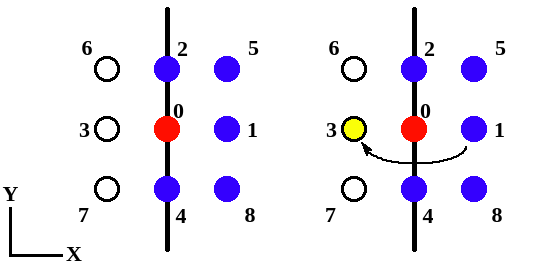
\includegraphics[width=0.85\textwidth]{figs/cap2/CC_hidrodinamica.png}
	\caption{Bloques de threads organizados en una grilla de bloques \cite{rinaldi2011modelos}.}
	\label{fig:CC_hidro}
\end{figure}

Por convención las direcciones que se conocen los valores de las funciones de distribución pertenecen al conjunto A y las que no se conocen al conjunto B. Por lo que $ 0, 1, 2, 4, 5, 8 \in A$ y $ 3, 6, 7 \in B$ 


\subsubsection{Condición hidrodinámica}

El desarrollo de Zou \cite{zou1997pressure} es el utilizado para la ecuación hidrodinámica. Primeramente el método \textit{bounceback} es aplicado a la dirección \textit{3}, resultando $f_{3} = f_{1}$ como se observa en la Figura \ref{fig:CC_hidro}. Luego se analizan las Ec. (\ref{eq:rho}) y (\ref{eq:U}) que son puestas de la siguiente forma:

\begin{equation}
	\begin{array}{c}
	f_{3} + f_{6} + f_{7} = \rho - \left( f_{0} + f_{1} + f_{2} + f_{4} + f_{5} + f_{8}	 \right)\\
	f_{6} - f_{7} = \rho u_{x} - \left( f_{1} - f_{3} - f_{7} + f_{8} 	 \right)\\
	f_{3} + f_{6} + f_{7} = \rho u_{y} + \left( f_{1} + f_{5} + f_{8} \right)
	\end{array}
\end{equation}

Para finalizar se aplican las condiciones de no deslizamiento, para éste caso $\> u_{y} = 0\quad$ y $\quad\mu \frac{\partial u}{\partial x} = \tau_{wall}\quad$, siendo $\tau_{wall}$ el esfuerzo de corte realizado en la arista analizada. Se obtenienen las siguientes condiciones de contorno a la distribución de poblaciones $\mathbf{f}$:

\begin{equation}
\begin{array}{c}
f_{i3} = f_{i1}\\
f_{i7} = f_{i5} - 0,5 (f_{i4} - f_{i2}) - 0,25 (F_{ix} + F_{iy})\\
f_{i6} = f_{i8} + 0,5 (f_{i4} - f_{i2}) - 0,25 (F_{ix} + F_{iy})\\
\end{array}
\end{equation}

donde el índice \textit{i} indica que es el nodo \textit{i}-ésimo que de la arista y $F_{ix}$, $F_{iy}$ es la fuerza del nodo. 


\subsubsection{Condición de energía}

La condición de contorno a realizar en la ecuación de energía, es mantener una temperatura fija en una de las aristas o en secciones de la misma. Por lo cual se utiliza el desarrollo de Inamuro \cite{inamuro2002lattice}.

Primeramente se calcula el valor de la distribución de equilibrio del nodo $i$-ésimo $\mathbf{g}_{eq\>i}$ utilizando Ec. (\ref{eq:n_eq}) y $\mathbf{M}$ de la forma $\mathbf{g_{eq}} = \mathbf{M}^{-1} \mathbf{n_{eq}}$. Se prosigue a calcular el parámetro $\beta$:

\begin{equation}
\beta = \frac{T_{cc} - \sum_{A} g_{A}}{\sum_{B} g_{B}}
\label{eq:beta}
\end{equation}

donde $T_{cc}$ es la temperatura fijada como condición de contorno, $g_{A}$ adopta los valores conocidos de las direcciones pertenecientes al cpnjunto A ($0, 1, 2, 4, 5, 8 $), mientras que $g_{B}$ adopta los valores de la dirección de $\mathbf{g_{eq}}$ calculada recientemente para las direcciones de B ($3, 6, 7$).

Por último en las direcciones del conjunto B, el valor de $g$ resulta:

\begin{align}
	g_{B} = \beta \> g_{eq \> B} 
\end{align}

A modo de ejemplo se detalla el valor que adoptará la dirección \textbf{3}:

\begin{equation}
	g_{3} = \frac{T_{cc} - \overbrace{\left( g_{0} + g_{1} +g_{2} + g_{4} + g_{5} + g_{8} \right)}^{\sum_{A} g_{A}} }{\underbrace{\left( g_{eq\>3} + g_{eq\>6} + g_{eq\>7} \right)}_{\sum_{B} g_{B} }} \quad g_{eq\>3}
\end{equation}


%%% Local Variables: 
%%% mode: latex
%%% TeX-master: "template"
%%% End: 

%\chapter{Implementación del código numérico en GPU}
\chapter{Código numérico de LBM}
\graphicspath{{figs/cap3/}}
\label{cap3}



%\section{Implementación del código}

En el presente capítulo se realizará la descripción de la implementación del código numérico del LBM descripto en la Sec. (\ref{sec:LBM_2_ec_MRT}), como también las implicancias de elaborar la implementación en una GPU de forma eficiente.

El lenguaje de programación \textsc{C} desarrollado por Dennis MacAlistair Ritchie será utlizado para desarrollar el código. Dicho lenguaje brinda instrucciones a la CPU de una PC para ser ejecutadas. Las CPU son diseñadas óptimamente para que sus instrucciones sean procesadas de forma secuencial en los núcleos que poseen; aunque también se permite realizar los procesos en paralelo, según la cantidad de núcleos.

Luego se implementará un código en \textsc{Cuda C}, desarrollado por la empresa NVIDIA. Este lenguaje permite ejecutar instrucciones en una GPU, la cual está diseñada para que los procesos a realizar sean de forma paralela.

Se eligió la programación en \textsc{C} y \textsc{Cuda C} para comparar la eficiencia en el tiempo de cálculo, debido a que el lenguaje \textsc{Cuda C} es una extensión del lenguaje \textsc{C}. La diferencia principal es que \textsc{Cuda C}  tiene una forma particular de escribir las funciones que se ejecutarán en la GPU, las cuales son llamadas \textit{kernel}.

Ambos códigos, en \textsc{C} y \textsc{Cuda C}, son compilados mediante \textsc{CMake} en bibliotecas tipo \textit{shared} y \textit{static} respectivamente. También se realizó la compilación en formato \textsc{ptx} de los \textit{kernels} de \textsc{Cuda C}, donde éste formato puede utilizarse en el lenguaje de programación interpretado \textsc{Python}. El módulo de \textsc{Python} necesario para adquirir los \textit{kernels} es \textsc{PyCuda}.

La implementación en \textsc{Python} es debido a su facilidad de programación, el cual permite incorporar las bibliotecas compiladas en otros lenguajes y así obtener una mayor versatilidad de problemas a resolver. \textsc{Python} puede ser utilizado en distintos sistemas oparativos como \textit{Linux}, \textit{Windows} y \textit{Mac OS}. 

Para visualizar los resultados del código se utiliza el programa \textsc{Paraview}, de modo que el formato que se eligió para la escritura de los campos es \textsc{Ensight Gold}. A través del lenguaje \textsc{C}, es que se hicieron las funciones de escritura de éste tipo de archivos y así observar gráficamente las variables de interés del problema que se desea resolver. El módulo \textsc{CTypes} de \textsc{Python} es la necesaria para adquirir las funciones de escritura de \textsc{Ensight} del código compilado en \textsc{C}.



\section{Programación en GPU}
\label{sec_pc}

Una computadora (\textit{Personal Computer} o PC) posee como procesador principal la CPU, cuyo diseño se encuentra optimizado para realizar tareas secuenciales. Comercialmente vienen de una amplia variedad de núcleos, en el rango de 8 a 64 núcleos en el caso de los Procesadores AMD Ryzen™ Threadripper, 4 a 8 núcleos en los Procesador AMD FX™, en el caso de Intel se encuentra el Procesador Intel® Core™ serie X con 18 núcleos y  Intel® Core™ I7-3770 de 4 núcleos entre otros. \cite{edp:2020:amd} \cite{icp:2020:intel}

Es posible realizar tareas y procesos en paralelo en la CPU proveyendo instrucciones a cada núcleo del procesador de forma independiente, siendo más eficiente en el tiempo de ejecución de los procesos realizados.

A su vez una PC opcionalmente puede contener un coprocesador siendo una GPU. Dicha placa se encuentra diseñada para realizar operaciones en paralelo, realizándolas en varios hilos de ejecución (\textit{threads}).




El procesador principal que tiene una PC es la CPU, por lo cual se denomina \textit{host}, la GPU es un coprocesador y se denomina \textit{device}. Las ejecuciones de los procesos en la CPU están diseñadas para que se efectúen de manera secuencial, en cuánto las de la GPU en paralelo; las últimas realizándose en varios hilos de ejecución (\textit{threads}). El nombre que recibe una función que ejecuta un proceso de forma paralela en la GPU se denomina \textit{kernel}. \textit{Host} y \textit{device} poseen su propia memoria RAM, llamadas \textit{host memory} y \textit{device memory} respectivamente. \cite{rinaldi2011modelos}

Los \textit{threads} que posee una GPU se pueden agrupar de dos formas, una de ellas es por bloques (\textit{thread block}) y la otra mediante grilla de bloques (\textit{grid}). Todos los \textit{threads} del mismo \textit{thread block} poseen un acceso rápido a una memoria compartida y permite sincronizar las ejecuciones que se les asigna. Debido a la posibilidad de sincronización de los mismos, se evita el riesgo de que varios \textit{threads} accedan de manera simultánea al mismo lugar de memoria. Un \textit{grid} es un conjunto de \textit{thread block}, en dónde las instrucciones del \textit{kernel} son paralelizadas, ésto vence la limitación de hardware del finito número de \textit{threads} por bloque. Puesto que la ejecución del proceso en los \textit{thread blocks} de un \textit{grid} pueden ser ejecutados en tiempos distintos, es necesario realizar un sincronización entre los mismos para que su comunicación sea segura y no haya conflictos\cite{tolke2010implementation}. La figura \ref{fig:block_grid_threads} muestra el concepto de \textit{grid} y \textit{thread block}.

\newpage
\begin{figure}[h!]
	\centering
	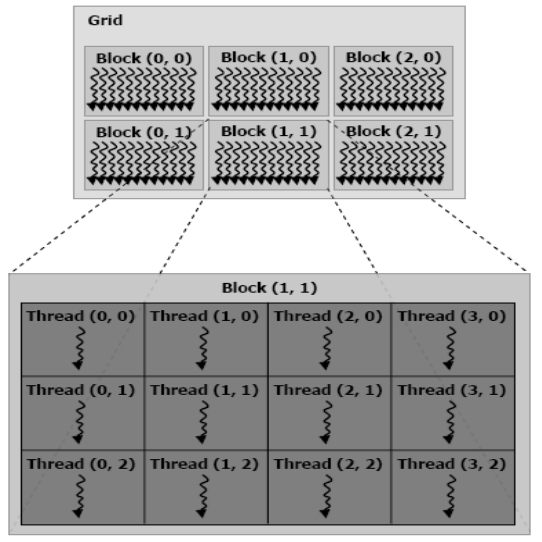
\includegraphics[width=0.4\textwidth]{figs/cap3/threads_block_grid.jpg}
	\caption{\textit{Thread blocks} organizados en un \textit{grid} \cite{rinaldi2011modelos}.}
	\label{fig:block_grid_threads}
\end{figure}

En el proyecto se utilizaron dos PC, cada una con distinta CPU y GPU. En la Tabla (\ref{tab:icore_gtx}) se encuentran las características de cada componente. La primera PC contaba con la CPU Intel Core i7-3770 y la GPU NVIDIA GeForce GTX 760. La segunda PC contaba con la CPU Intel Core i7-4770 y la GPU NVIDIA GeForce GTX 970.

\begin{table}[h!]
	\resizebox{\textwidth}{!}{
	\begin{tabular}{|c|c|c|cccc}
		\cline{1-3} \cline{5-7}
		Intel Core                                                                     & i7-3770        & i7-4770        & \multicolumn{1}{c|}{} & \multicolumn{1}{c|}{NVIDIA GeForce}                                                                        & \multicolumn{1}{c|}{GTX 760}       & \multicolumn{1}{c|}{GTX 970}       \\ \cline{1-3} \cline{5-7} 
		Núcleos                                                                        & 4              & 4              & \multicolumn{1}{c|}{} & \multicolumn{1}{c|}{Núcleos CUDA}                                                                          & \multicolumn{1}{c|}{1152}          & \multicolumn{1}{c|}{1664}          \\ \cline{1-3} \cline{5-7} 
		Threads                                                                        & 8              & 8              & \multicolumn{1}{c|}{} & \multicolumn{1}{c|}{\begin{tabular}[c]{@{}c@{}}Frecuencia de \\ reloj normal {[}MHz{]}\end{tabular}}       & \multicolumn{1}{c|}{980}           & \multicolumn{1}{c|}{1050}          \\ \cline{1-3} \cline{5-7} 
		\begin{tabular}[c]{@{}c@{}}Frecuencia de \\ base {[}GHz{]}\end{tabular}        & 3,40           & 3,40           & \multicolumn{1}{c|}{} & \multicolumn{1}{c|}{Tipo de Memoria}                                                                       & \multicolumn{1}{c|}{GDDR5 a 6 GHz} & \multicolumn{1}{c|}{GDDR5 a 7 GHz} \\ \cline{1-3} \cline{5-7} 
		\begin{tabular}[c]{@{}c@{}}Tamaño de \\ memoria caché {[}MB{]}\end{tabular}    & 8              & 8              & \multicolumn{1}{c|}{} & \multicolumn{1}{c|}{\begin{tabular}[c]{@{}c@{}}Configuracion de \\ memoria estándar {[}MB{]}\end{tabular}} & \multicolumn{1}{c|}{2048}          & \multicolumn{1}{c|}{4096}          \\ \cline{1-3} \cline{5-7} 
		Tipo de Memoria                                                                & DDR3-1333/1600 & DDR3-1333/1600 & \multicolumn{1}{c|}{} & \multicolumn{1}{c|}{Interfaz de Memoria {[}bits{]}}                                                        & \multicolumn{1}{c|}{256}           & \multicolumn{1}{c|}{256}           \\ \cline{1-3} \cline{5-7} 
		Tamaño de Memoria {[}GB{]}                                                     & 32             & 32             & \multicolumn{1}{c|}{} & \multicolumn{1}{c|}{\begin{tabular}[c]{@{}c@{}}Ancho de banda \\ de memoria {[}GB/s{]}\end{tabular}}       & \multicolumn{1}{c|}{192.2}         & \multicolumn{1}{c|}{224.0}         \\ \cline{1-3} \cline{5-7} 
		\begin{tabular}[c]{@{}c@{}}Ancho de banda\\ de memoria {[}GB/s{]}\end{tabular} & 25,6           & 25,6           &                       &                                                                                                            &                                    &                                    \\ \cline{1-3}
	\end{tabular}}
	\caption{Especificaciones técnicas de las CPU y GPU utilizadas \cite{i73:2020:intel}\cite{i74:2020:intel}\cite{760:2020:nvidia}\cite{970:2020:nvidia}.}
	\label{tab:icore_gtx}
\end{table}


\section{Arquitectura de la memoria de una GPU}

\begin{figure}[h!]
	\centering
	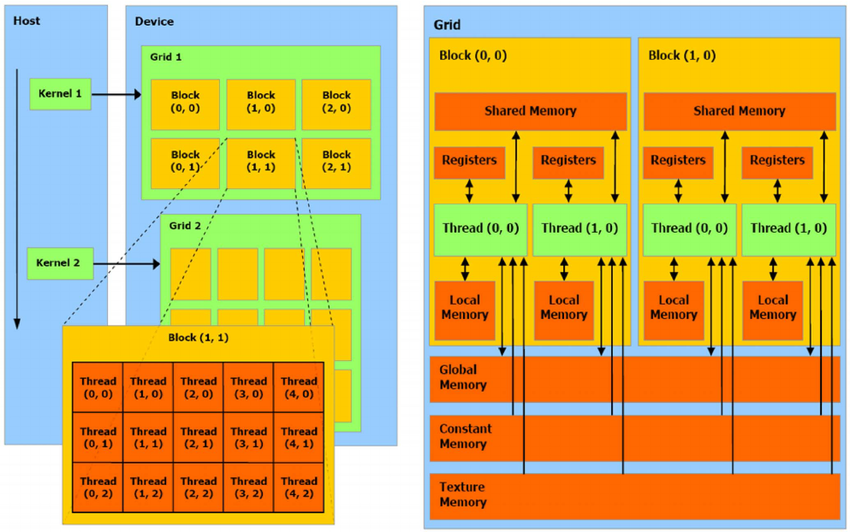
\includegraphics[width=\textwidth]{figs/cap3/Schematization-of-CUDA-architecture-Schematic-representation-of-CUDA-threads-and-memory.png}
	\caption{Esquematización de la arquitectura de CUDA. Izquierda: lanzamiento de un \textit{kernel} desde el \textit{host}. Derecha: jerarquía de memoria.  \cite{nobile2014cutauleaping}.}
	\label{fig:schedule_architecture_cuda}
\end{figure}

Según la arquitectura que posea un procesador, con su respectiva jerarquía en memoria, accesos y latencias, se planifica cómo llevar a cabo la implementación de un código, por ello es de importancia conocer dichas características. 

Anteriormente se mencionó que el \textit{host} y \textit{device} poseen su propia memoria. La transferencia de datos de una memoria a otra tiene una muy alta latencia en cualquiera de los dos sentidos; por lo que al diseñar un código, hay que minimizar la transferencia de datos entre los dos tipos de memoria, y así obtener el menor tiempo de ejecución de los procesos.

Cuando el \textit{host} efectúa su rutina de ejecución y se encuentra con un lanzamiento de \textit{kernel}, éste será llevado a cabo en múltiples \textit{threads} del \textit{device}. Una representación de ello se muestra en la figura \ref{fig:schedule_architecture_cuda}. 

Los procesos en el \textit{device} tienen almacenados los datos según una jerarquía de memoria, con su respectiva limitación de acceso que se observa en la figura \ref{fig:schedule_architecture_cuda}. Los \textit{threads} pueden acceder a datos de muchas memorias diferentes en distintos procesos, dichas memorias son las siguientes:

\begin{itemize}
	\item  \textit{register memory} es visible para un único \textit{thread}
	\item \textit{local memory} tiene las mismas caracteísticas que \textit{register memory} pero con una performance menor.
	\item \textit{shared memory} es visible por todos los \textit{threads} de un mismo bloque, posee una baja latencia en su acceso.
	\item \textit{global memory} es visible por todos los \textit{threads} de la grilla y también por el \textit{host}, posee una alta latencia de acceso.
	
	Las siguientes memorias poseen una alta latencia de acceso son asignadas y son aignadas para usos específicos y generalmente se almacenan en \textit{caché}:
	
	\item \textit{constant memory} es visible por todos los \textit{threads} de la grilla siendo únicamente de lectura. El uso de ésta memoria puede reducir el ancho de banda de memoria requerido en comparación con la {global memory}
	\item \textit{texture memory} es otra memoria en la que sólo se puede leer y tienen acceso todos los \textit{threads} de la grilla. Al realizar lecturas de \textit{threads} ó \textit{threadblocks} adyacentes su performance en comparación con \textit{global memory} es mayor. 
	
\end{itemize}


\section{Programación en CUDA C}

La programación de las GPU se lleva a cabo mediante el lenguaje \textsc{Cuda C}, el cual es una extención del lenguaje \textsc{C} debido su familiaridad y uso extendido; por lo que el lenguaje se denomina \textsc{Cuda C}. La versión 10.1 de CUDA fue la utilizada para el desarrollo del presente trabajo. La realización de procesos en paralelos es ejecutada mediante funciones llamadas \textit{kernel} y son del tipo \textit{void}.
\\

Existen tres tipos de funciones que se pueden efectuar en \textsc{Cuda C} y son:

\begin{itemize}
	
	\item \textbf{host} función clásica de C que se ejecuta en la CPU, siendo invocable únicamente por funciones que se realicen en la CPU. 

	\item \textbf{global} es una función \textit{kernel} invocada desde la CPU para ejecutarse en la GPU. 
%	Debe especificar la cantidad de bloques y de \textit{threads} por bloque a lanzar la función.
	
	\item \textbf{device} es una función que se ejecuta en la GPU y únicamente puede ser llamada desde un \textit{kernel}.
	
\end{itemize}

En el presente trabajo sólo se utilizaran funciones de tipo \textbf{host} y \textbf{global}, pudiéndose realizar en un futuro el  \textit{profiling} mediante el uso de las funciones tipo \textbf{device}.

Otra particularidad que se presenta en la programación es el manejo de la memoria por parte del \textit{host} como del \textit{device}, siendo abordado posteriormente.


\subsection{Programación de un \textit{kernel}}

Para visualizar las diferencias de programación de una función \textbf{CUDA C } (\textit{kernel}), con una típica función de \textsc{C}, se muestra a continuación como ejemplo la programación para ambos lenguajes de la Ec. (\ref{eq:rho})


En primer lugar se detalla el código realizado en el lenguaje \textsc{C}, siendo la función :

{\footnotesize
	\begin{frame}{}
		\lstset{language=C,
			framesep=2mm,
			basicstyle=\ttfamily,
			keywordstyle=\color{blue}\ttfamily,
			stringstyle=\color{red}\ttfamily,
			commentstyle=\color{green}\ttfamily,
			morecomment=[l][\color{magenta}]{\#}
		}
		\begin{lstlisting}
void momentoDensity(scalar* rho, scalar* field, basicMesh* mesh);
		\end{lstlisting}
		
	\end{frame}
}.
\\
donde el argumento \textbf{basicMesh* mesh} es un puntero a una estructura, la cual posee información del mallado que se realizó al dominio del problema a resolver, como por ejemplo la cantidad de nodos que posee la malla (\textbf{nPoints}) y la cantidad de direcciones que posee el modelo en su espacio de velocidades \textbf{Q}. La variable \textbf{scalar} corresponde a una de tipo \textcolor{blue}{float} o \textcolor{blue}{double}, según opciones elegidas al momento de la compilación. El \textit{array}  \textbf{scalar* rho} es de dimensión \textit{nPoints} y contiene los valores de $\rho$, por último \textbf{scalar* field} es un \textit{array} que posee las \textit{q} componentes de la función de distribución de poblaciones \textit{f} para cada uno de los  \textit{nPoints} nodos de la malla.


{\footnotesize
	\begin{frame}{}
		\lstset{language=C,
			framesep=2mm,
			basicstyle=\ttfamily,
			keywordstyle=\color{blue}\ttfamily,
			stringstyle=\color{red}\ttfamily,
			commentstyle=\color{green}\ttfamily,
			morecomment=[l][\color{magenta}]{\#}
		}
		\begin{lstlisting}[frame=single]
#include <momentoDensity.h>
#include <stdio.h>

void momentoDensity(scalar* rho, scalar* field, basicMesh* mesh) {
	
	// Suma de todas las componentes
	
	for( uint i = 0 ; i < mesh->nPoints ; i++ ) {
		
		rho[i] = 0;	    
		
		for( uint j = 0 ; j < mesh->Q ; j++ ) {
		
			rho[i] += field[ i*mesh->Q + j ];
		
		}	
			
	}
	
}
		\end{lstlisting}
		
	\end{frame}
}.
\\

La programación de la Ec.(\ref{eq:rho}) implementada en \textsc{Cuda C} es con el \textit{kernel}:

{\footnotesize
	\begin{frame}{}
		\lstset{language=C,
			framesep=2mm,
			basicstyle=\ttfamily,
			keywordstyle=\color{blue}\ttfamily,
			stringstyle=\color{red}\ttfamily,
			commentstyle=\color{green}\ttfamily,
			morecomment=[l][\color{magenta}]{\#}
		}
		\begin{lstlisting}
extern "C" __global__ void cudaMomentoDensity(
	cuscalar* field,cuscalar* rho, int np, int Q ) ; 
		\end{lstlisting}
		
	\end{frame}
}.
\\
en este caso se pasa de forma distinta los valores de la cantidad de nodos (\textit{np}) y de la cantidad de velocidades del modelo \textit{DdQq} (\textit{Q}). La distinción en los argumentos que se pasan en ambos códigos, es debido a la forma que \textsc{Cuda C} permite el manejo de las estructuras y también de las decisiones que se tomaron cuando se desarrollaba el código para uno u otro lenguaje.

Se coloca \textcolor{blue}{extern} \textcolor{red}{''C''} para que el compilador detecte que es un \textit{kernel} de \textsc{Cuda C} y cuando se le indique pueda compilar los \textit{kernel} en formato \textsc{ptx}.

\newpage

{\footnotesize
	\begin{frame}{}
		\lstset{language=C,
			framesep=2mm,
			basicstyle=\ttfamily,
			keywordstyle=\color{blue}\ttfamily,
			stringstyle=\color{red}\ttfamily,
			commentstyle=\color{green}\ttfamily,
			morecomment=[l][\color{magenta}]{\#}
		}
		\begin{lstlisting}[frame=single]
#include <cudaMomentoDensity.h>
#include <cuda_runtime.h>
#include <stdio.h>
#include <stdlib.h>

extern "C" __global__ void cudaMomentoDensity(cuscalar* field,
				              cuscalar* rho,
					      int np,
					      int Q ) {
							
	int idx = threadIdx.x + blockIdx.x*blockDim.x;	
	
	if( idx < np ) {	
	
		int j= 0;		
	
		cuscalar sum = 0;		
	
		while ( j < Q ) {		
	
			sum += field[ idx*Q + j ];			
	
			j++;			
	
		}				
	
		rho[idx] = sum;	
	
	}
	
}		
		\end{lstlisting}
		
	\end{frame}
}.
\\
%en este leguaje, se observó que es más eficiente el uso de la función \textcolor{blue}{\textbf{while}} que \textcolor{blue}{\textbf{for}} en el tiempo de ejecución del código.

Es de importancia conocer la función que cumplen las siguientes líneas:
{\footnotesize
	\begin{frame}{}
		\lstset{language=C,
			framesep=2mm,
			basicstyle=\ttfamily,
			keywordstyle=\color{blue}\ttfamily,
			stringstyle=\color{red}\ttfamily,
			commentstyle=\color{green}\ttfamily,
			morecomment=[l][\color{magenta}]{\#}
		}
		\begin{lstlisting}
	int idx = threadIdx.x + blockIdx.x*blockDim.x;	
	if( idx < np ) {	
		\end{lstlisting}
		
	\end{frame}
}.
\\
donde las tareas que se hallen en \textcolor{blue}{if} ( idx < np)\{...\} se realizarán de forma paralela y es necesario identificar los \textit{threads} en dónde se llevaran a cabo los procesos. El identificador de los \textit{threads} es \textit{idx} donde blockIdx.x  indica la cantidad de \textit{threads} por \textit{block} y blockDim.x el numero de \textit{block's}.

Resta ver cómo es el llamado de las funciones realizadas en el \textit{main}, por lo que en \textsc{C} se observa:


{\footnotesize
	\begin{frame}{}
		\lstset{language=C,
			framesep=2mm,
			basicstyle=\ttfamily,
			keywordstyle=\color{blue}\ttfamily,
			stringstyle=\color{red}\ttfamily,
			commentstyle=\color{green}\ttfamily,
			morecomment=[l][\color{magenta}]{\#}
		}
		\begin{lstlisting}
		momentoDensity( rho, field_f, &mesh);
		\end{lstlisting}
		
	\end{frame}
}.
\\
la cual no requiere de ninguna explicación, mientras que en \textsc{Cuda C} se tiene:

{\footnotesize
	\begin{frame}{}
		\lstset{language=C,
			framesep=2mm,
			basicstyle=\ttfamily,
			keywordstyle=\color{blue}\ttfamily,
			stringstyle=\color{red}\ttfamily,
			commentstyle=\color{green}\ttfamily,
			morecomment=[l][\color{magenta}]{\#}
		}
		\begin{lstlisting}
cudaMomentoDensity<<<ceil(mesh.nPoints/xgrid)+1,xgrid>>>(
 		deviceField, deviceRho, cmesh.nPoints, cmesh.Q);  
cudaDeviceSynchronize();

		\end{lstlisting}
		
	\end{frame}
}.
\\
en donde < < <, > > > indica la cantidad de \textit{thread blocks} en que se realizará la tarea, como así también la cantidad de \textit{threads} en cada \textit{block}.

\begin{align*}
		<<<\quad \overbrace{ceil(mesh.nPoints/xgrid)+1}^{cantidad \>de\> \textit{threads}\> por\> \textit{block}}\quad,\quad \underbrace{xgrid}_{cantidad\>de\>thread\>block} \quad>>>
\end{align*}

\subsection{Sincronización}

Debido a que los procesos en la GPU son asignados de una forma no determinística, es necesario que exista un procedimiento para sincronizar los \textit{threads}. Por ejemplo, un conflicto puede ser que el Thread idx = 1 quiera acceder a un lugar de la memoria al mismo tiempo que el Thread idx = 2. Otro caso es que el Thread idx = 1 escriba un valor en la \textit{global memory} y se requiera que el Thread idx = 2 realice alguna operación con dicho valor. El método utilizado para resolver éstos problemas es \textbf{cudaDeviceSynchronize()}, el cual sincroniza los \textit{thread blocks} de una \textit{grid}.

\subsection{Utilización de la memoria de \textit{host} y \textit{device}}


Las funciones que son realizadas en \textsc{C} permiten retornar alguna variable mientras que en \textsc{Cuda C} los \textit{kernel} son del tipo \textit{void}, debido a ello es necesario almacenar memoria en el \textit{device} para una variable, y pasarla como argumento al \textit{kernel}. Lo mencionado permite que el \textit{kernel} modifique dicha variable y así obtener lo requerido. 

La allocación de memoria en el \textit{host} es la misma que se utiliza en \textsc{C}  \textbf{malloc($\>$)} :
{\footnotesize
	\begin{frame}{}
		\lstset{language=C,
			framesep=2mm,
			basicstyle=\ttfamily,
			keywordstyle=\color{blue}\ttfamily,
			stringstyle=\color{red}\ttfamily,
			commentstyle=\color{green}\ttfamily,
			morecomment=[l][\color{magenta}]{\#}
		}
		\begin{lstlisting}
		void *malloc(size_t size)
		\end{lstlisting}
		
	\end{frame}
}.
\\
siendo \textit{size\_t} la memoria en bytes a reservar. Mientras que en el \textit{device} se realiza por medio de \textbf{cudaMalloc($\>$)} :
\\
{\footnotesize
\begin{frame}{}
	\lstset{language=C,
		framesep=2mm,
		basicstyle=\ttfamily,
		keywordstyle=\color{blue}\ttfamily,
		stringstyle=\color{red}\ttfamily,
		commentstyle=\color{green}\ttfamily,
		morecomment=[l][\color{magenta}]{\#}
	}
	\begin{lstlisting}
		cudaMalloc(void **devPtr, size_t size);
	\end{lstlisting}

\end{frame}
}.
\\
donde \textit{devPtr} es un puntero para allocar la memoria del \textit{device} , \textit{size\_t} memoria en bytes a reservar. Se debe tener en cuenta que la memoria se reserva linealmente.

La transferencia de datos entre los dos tipos de memoria se efectua mediante la función \textbf{cudaMemcpy($\>$)} :
{\footnotesize
\begin{frame}{}
	\lstset{language=C,
		framesep=2mm,
%		baselinestretch=1.2,
		basicstyle=\ttfamily,
		keywordstyle=\color{blue}\ttfamily,
		stringstyle=\color{red}\ttfamily,
		commentstyle=\color{green}\ttfamily,
		morecomment=[l][\color{magenta}]{\#}
	}
	\begin{lstlisting}
cudaMemcpy(void *dst, void *src, size_t count, cudaMemcpyKind kind);
	\end{lstlisting}
	
\end{frame}
}.
\\
siendo \textit{dst} un puntero con la dirección de destino de los datos, \textit{src} un puntero con la dirección de origen de los datos, \textit{count} es la cantidad de bytes a transferir y \textit{kind} es el tipo de transferencia a realizar \cite{zone2020cuda}. La tabla \ref{tab:cudamemcy} contiene los cuatro tipos posibles de transferencia.


\begin{table}[h!]
\centering
	\centering
	\begin{tabular}{|c|c|}
		\hline
		\multicolumn{1}{|l|}{TIPO DE TRANSFEREMCIA} & \multicolumn{1}{l|}{SENTIDO DE TRANSFERENCIA} \\ \hline
		\textbf{cudaMemcpyHostToHost}               & \xymatrix{host\ar@^{->}[r]&host}              \\ \hline
		\textbf{cudaMemcpyHostToDevice}             & \xymatrix{host\ar@^{->}[r]&device}            \\ \hline
		\textbf{cudaMemcpyDeviceToHost}             & \xymatrix{device\ar@^{->}[r]&host}            \\ \hline
		\textbf{cudaMemcpyDeviceToDevice}           & \xymatrix{device\ar@^{->}[r]&device}          \\ \hline
	\end{tabular}
	\caption{Tipos de transferencias de datos en CUDA \cite{represa2016introduccion}.}
	\label{tab:cudamemcy}
\end{table}



\section{Programación en Python}

Habiéndose desarrollado el código en \textsc{Cuda C} y compilado cada \textit{kernel} del mismo en formato \textsc{ptx}, éstos pueden ser utilizados en el lenguaje \textsc{Python} mediante el módulo \textsc{PyCuda}. El código de la siguiente página es el implementado para la Ec. (\ref{eq:rho}).

Donde la función \textit{pycuda.driver.module\_from\_file()} nos permite importar el \textit{kernel} compilado previamente en \textsc{Cuda C}, siendo \textcolor{red}{\textbf{/PATH/}} la dirección del directorio dónde se encuentra el archivo \textsc{ptx} compilado. Las variables \textit{deviceField} y \textit{deviceRho} son las respectivas a la función de distribución de poblaciones \textit{f} y la densidad $\rho$. Previamente se deben haber inicializado las variables en el \textit{host}, como por ejemplo:
{\footnotesize
	\begin{frame}{}
		\lstset{language=python,
			framesep=2mm,
			%		baselinestretch=1.2,
			basicstyle=\ttfamily,
			keywordstyle=\color{blue}\ttfamily,
			stringstyle=\color{red}\ttfamily,
			commentstyle=\color{green}\ttfamily,
			morecomment=[l][\color{magenta}]{\#}
		}
		\begin{lstlisting}
	hostField = numpy.zeros( nPoints*meshQ, dtype=np.float32 ) 
		\end{lstlisting}
		
	\end{frame}
}.
\\
y luego ser copiadas y allocadas en el  \textit{device} con la función \textit{gpuarray.to\_gpu()} :
{\footnotesize
	\begin{frame}{}
		\lstset{language=python,
			framesep=2mm,
			%		baselinestretch=1.2,
			basicstyle=\ttfamily,
			keywordstyle=\color{blue}\ttfamily,
			stringstyle=\color{red}\ttfamily,
			commentstyle=\color{green}\ttfamily,
			morecomment=[l][\color{magenta}]{\#}
		}
		\begin{lstlisting}
		deviceField = gpuarray.to_gpu( hostField )
		\end{lstlisting}
		
	\end{frame}
}.
\\
Además de los argumentos que tenía originalmente el \textit{kernel}; hay que pasarle a la función obtenida por \textsc{PyCuda} el número de \textit{blocks} \textbf{block=( args.xgrid, 1, 1 )} y la cantidad de \textit{thread por block} \textbf{grid=( gs, 1, 1)} donde será ejecutada. 

Por último la sincronización de los \textit{threads} es proporcionada mediante el método \\
\textit{pycuda.driver.Context.synchronize()}.

{\footnotesize
	\begin{frame}{}
		\lstset{language=python,
			framesep=2mm,
			%		baselinestretch=1.2,
			basicstyle=\ttfamily,
			keywordstyle=\color{blue}\ttfamily,
			stringstyle=\color{red}\ttfamily,
			commentstyle=\color{green}\ttfamily,
			morecomment=[l][\color{magenta}]{\#}
		}
		\begin{lstlisting}[frame=single]
import pycuda
from pycuda import gpuarray
import pycuda.autoinit
		
cudaMomentoDensity = pycuda.driver.module_from_file(
			'/PATH/cudaMomentoDensity.ptx').get_function(
			'cudaMomentoDensity')					
cudaMomentoDensity(	deviceField,
			deviceRho,
			mesh.nPoints,
			mesh.Q,
			block=( args.xgrid, 1, 1 ),
			grid=( gs, 1, 1) )     			    
pycuda.driver.Context.synchronize()
		\end{lstlisting}
		
	\end{frame}
}




	   

\section{Arquitectura del código numérico y compilación}

El código numérico fue desarrollado en el repositorio de la página web \textsc{Git Hub}, la cual permite realizar un control de versiones. En la Sec.(\ref{sec:git}) se explica conceptos básicos para utilizar la herramienta \textsc{Git}, las funciones más relevantes y buenas prácticas que se adquirieron en el transcurso del presente trabajo. El proyecto se encuentra disponible para ser descargado en \url{https://github.com/efogliatto/LBCUDA_Test}, siendo la carpeta LBCUDA\_Test la que contiene el proyecto. La versión 1.0 de la rama \textit{master} es la que se poseía al momento de finalizar el presente trabajo.

Las subcarpetas (\textbf{en negrita}) y archivos (\underline{subrayados}) que posee nuestro proyecto en su directorio principal son los siguientes:

\begin{itemize}
	\item \textbf{build}: es el directorio de construcción, desde el cuál se compila el proyecto.
	
	\item \textbf{bin}: es el directorio en el cual se encuentran los ejecutables del proyecto.
	
	\item \textbf{include}: es el directorio en el cual se encuentran los \textit{links} simbólicos a todos los \textit{headers} de las funciones y \textit{kernels} realizados.
	
	\item \textbf{lib}: es el directorio en el cual, una vez compilado el proyecto, se encuentran las bibliotecas realizadas en \textsc{C} y \textsc{Cuda C}.
	
	\item \textbf{ptx}: es el directorio en el cual, una vez compilado el proyecto, se encuentran compilados los \textit{kernel} de \textsc{Cuda C} en formato \textsc{ptx}.	
	
	\item \textbf{src}: es el directorio que posee los códigos fuente para los lenguajes \textsc{C}, \textsc{Cuda C} y \textsc{Python}.
	
	\item \textbf{examples}: es el directorio el cual posee ejemplos de ejecución del código por medio de \textit{scripts} de bash.
	
	\item \textbf{validation\_speed\_up}: es un directorio que contiene dos tipos de \textit{scripts} de bash. Los del primer tipo al ser ejecutados, realizan la validación de los problemas tratados en el Cap. (\ref{cap4}). El otro tipo de \textit{scripts} realizan una toma de tiempo de cálculo de los mismos problemas, para obtener un índice (\textit{speed\_up}) que indique la mejora de tiempo de cálculo entre lenguajes utilizados. 
	
	\item \underline{CMakeLists.txt}: es el archivo principal del compilador utilizado, el cual contiene todas las opciones de compilación del proyecto.
	
\end{itemize}


La herramienta de software \textsc{CMake} fue la utilizada para compilar el código desarrollado,  donde el archivo CMakeLists.txt principal tiene que encontrarse en la carpeta principal del proyecto \cite{cmake:2020:kitware}. Dicho archivo contiene todas las instrucciones de compilación que debe/puede tener un proyecto a trabajar. A continuación se detallan las instrucciones más relevantes.

Para indicar las carpetas de construcción (\textit{build}), ejecutables (\textit{bin}), bibliotecas (\textit{lib}), \textit{headers} de las funciones y \textit{kernels} (\textit{include}) y código fuente (\textit{src}) se incorporan las siguientes instrucciones:

%, algunas de ellas son los directorios en que se encuentran los binarios, ejecutables, bibliotecas, códigos fuente entre otros. Otra de las instrucciones son los lenguajes a compilar con sus respectivas opciones de compilación. A continuación se describe las instrucciones ed compilación que tuvo el proyecto.


{\footnotesize
	\begin{frame}{}
		\lstset{language=c,
			framesep=2mm,
			%		baselinestretch=1.2,
			basicstyle=\ttfamily,
			keywordstyle=\color{blue}\ttfamily,
			stringstyle=\color{red}\ttfamily,
			commentstyle=\color{green}\ttfamily,
			morecomment=[l][\color{magenta}]{\#}
		}
		\begin{lstlisting}[frame=single]
	set(CMAKE_BINARY_DIR ${CMAKE_SOURCE_DIR}/build)

	set(EXECUTABLE_OUTPUT_PATH ${CMAKE_SOURCE_DIR}/bin)

	set(LIBRARY_OUTPUT_PATH ${CMAKE_SOURCE_DIR}/lib)

	include_directories(include) # Bring the headers
	
	add_subdirectory (src) 	# Directorio con fuentes

		\end{lstlisting}
		
	\end{frame}
}


Para asignar las bibliotecas en que se compilarán el código, se incorporan las instrucciones mostradas a continuación, donde se colocaron algunas bibliotecas utilizadas a modo de ejemplo.
\newpage
{\footnotesize
	\begin{frame}{}
		\lstset{language=c,
			framesep=2mm,
			%		baselinestretch=1.2,
			basicstyle=\ttfamily,
			keywordstyle=\color{blue}\ttfamily,
			stringstyle=\color{red}\ttfamily,
			commentstyle=\color{green}\ttfamily,
			morecomment=[l][\color{magenta}]{\#}
		}
		\begin{lstlisting}[frame=single]
# Link libraries

#Para el codigo realizado en C
set ( PROJECT_LINK_LIBS 
liblatticemodel.so 		
liblatticemesh.so
...
)

#Para el codigo realizado en Cuda C
set ( CUDATEST_LINK_LIBS 
cudatest.a
cudalatticemesh.a
...
)

link_directories( ${CMAKE_SOURCE_DIR}/lib )
		
		\end{lstlisting}
		
	\end{frame}
}

La instrucción de asignar opciones de compilación en \textsc{C} y \textsc{Cuda C} respectivamente son las siguientes :
\\\\
\textcolor{blue}{\textbf{SET}}( CMAKE\_C\_FLAGS  \textcolor{red}{''\$\{CMAKE\_C\_FLAGS\} (opciones)''})
\\\\
\textcolor{blue}{\textbf{SET}}( CMAKE\_CUDA\_FLAGS  \textcolor{red}{''\$\{CMAKE\_CUDA\_FLAGS\} (opciones)''})
\\
\\
donde es importante señalar que dependiendo de la aquitectura que posee la GPU, debe asignársele una distinta opción de compilación. A continuación su muestra una opción de compilación genérica, en donde xx se refiere a la arquitectura de la GPU.
\\
\\
\textcolor{blue}{\textbf{SET}}( CMAKE\_CUDA\_FLAGS \textcolor{red}{''\$\{CMAKE\_C\_FLAGS\}}\\
                 $.\qquad \qquad \qquad $\textcolor{red}{ -gencode arch=compute\_xx,code=sm\_xx -rdc=true''})
\\


Otras de las instrucciones que se le asignó al compilador, es que tenga la opción de que el proyecto se  compile únicamente en \textsc{C} ó, en su defecto  \textsc{C} y \textsc{Cuda C}. A su vez como se trabajó con distintas GPU, se implementó que el compilador detecte de forma automática la arquitectura que poseía la GPU de la PC, en dónde se está realizando la compilación. 

El siguiente archivo de configuración de \textsc{CMake} muestra la implementación de las instrucciones descriptas arriba:
\newpage

{\scriptsize
	\begin{frame}{}
		\lstset{language=c,
			framesep=2mm,
			%		baselinestretch=1.2,
			basicstyle=\ttfamily,
			keywordstyle=\color{blue}\ttfamily,
			stringstyle=\color{red}\ttfamily,
			commentstyle=\color{green}\ttfamily,
			morecomment=[l][\color{magenta}]{\#}
		}
		\begin{lstlisting}[frame=single]

SET( CMAKE_C_FLAGS  "${CMAKE_C_FLAGS} -Wall -lm -pedantic -funroll-loops" )

# Opcional: Desabilitar CUDA para poder compilar al menos
# una parte en dispositivos sin GPU

option(DISABLE_CUDA "Deshabilitar manualmente la compilacion en CUDA" OFF)

set(CUDAARCH "30" CACHE STRING "Arquitectura de GPU")

if(DISABLE_CUDA)

	# Asignar solo C como lenguaje de compilacion
	project(LBCUDA_Test LANGUAGES C)

else()
	# Asignar C y CUDA como lenguajes
	project(LBCUDA_Test LANGUAGES CUDA C)
	
	# Bibliotecas para compilar CUDA
	find_package( CUDA REQUIRED )

	# Opciones de compilador
	if(CUDAARCH STREQUAL "30")
		message("-- CUDA: Arquitectura 30")
		SET( CMAKE_CUDA_FLAGS  "${CMAKE_CUDA_FLAGS} 
				-gencode arch=compute_30,code=sm_30 -rdc=true")
	else()
		if(CUDAARCH STREQUAL "50")
			message("-- CUDA: Arquitectura 50")      
			SET( CMAKE_CUDA_FLAGS  "${CMAKE_CUDA_FLAGS} 
					-gencode arch=compute_50,code=sm_50 -rdc=true")
		else()
			message("-- CUDA: Arquitectura no reconocida. Uso de 30")
			SET( CMAKE_CUDA_FLAGS  "${CMAKE_CUDA_FLAGS} 
					-gencode arch=compute_30,code=sm_30 -rdc=true")      
		endif()
	endif()
endif()
		
		\end{lstlisting}
		
	\end{frame}
}

Por último el código numérico se realizó para que sus variables estén en simple precisión o doble precisión. Por lo cual en el código de \textsc{C}, la declaración de variables que tomarán la asignación de \textcolor{blue}{float} ó \textcolor{blue}{double} será \textbf{scalar}, mientras que en el código de \textsc{Cuda C} será \textbf{cuscalar}. 

La forma de concretar lo mencionado se realizó en dos partes. La primera de ellas es que en el CMakeLists.txt principal se declararon las variables SP, DP, SP\_CUDA y DP\_CUDA, correspondiendo a simple precisión, doble precisión en \textsc{C} y \textsc{Cuda C} respectivamente. Por lo que dependiendo de que variable es la adoptada en el compilador, será la que se utilice luego en el código. El archivo de configuración de \textsc{CMake} que ejecuta lo propuesto es el siguiente:

\newpage
{\scriptsize
	\begin{frame}{}
		\lstset{language=c,
			framesep=2mm,
			%		baselinestretch=1.2,
			basicstyle=\ttfamily,
			keywordstyle=\color{blue}\ttfamily,
			stringstyle=\color{red}\ttfamily,
			commentstyle=\color{green}\ttfamily,
			morecomment=[l][\color{magenta}]{\#}
		}
		\begin{lstlisting}[frame=single]
# Optional: precision
set(PRECISION "simple" CACHE STRING "Floating-point precision")

if(PRECISION STREQUAL "double")
	message("-- C   : Double precision")
	add_definitions(-DDP)

	elseif(PRECISION STREQUAL "simple")
		add_definitions(-DSP)
		message("-- C   : Simple precision")
	else()
		message( FATAL_ERROR "Precision not supported" )
endif()

# Optional: CUDA precision
set(CUDA_PRECISION "simple" CACHE STRING "CUDA Floating-point precision")

if(CUDA_PRECISION STREQUAL "simple")
	message("-- CUDA: Simple precision")
	add_definitions(-DSP_CUDA)

	elseif(CUDA_PRECISION STREQUAL "double")
		add_definitions(-DDP_CUDA)
		message("-- CUDA: Double precision")
	else()
		message( FATAL_ERROR "CUDA Precision not supported" )
endif()
		
		\end{lstlisting}
		
	\end{frame}
}
La segunda parte para asignar un tipo de variable a \textbf{scalar} y \textbf{cuscalar} es el \textit{script} de tipo \textit{header} que aparece debajo. En él se busca las variables declaradas en el compilador (SP, DP, SP\_CUDA ó DP\_CUDA) y en base a ellas, define el tipo de variable para \textbf{scalar} y \textbf{cuscalar}. El \textit{header}, cuyo nombre de archivo es \textit{dataTypes.h} y se encuentra en el directorio \textit{include}, debe ser incluido en cada función o \textit{kernel} que posea una variable de tipo  \textbf{scalar} o \textbf{cuscalar}.

{\footnotesize
	\begin{frame}{}
		\lstset{language=c,
			framesep=2mm,
			%		baselinestretch=1.2,
			basicstyle=\ttfamily,
			keywordstyle=\color{blue}\ttfamily,
			stringstyle=\color{red}\ttfamily,
			commentstyle=\color{green}\ttfamily,
			morecomment=[l][\color{magenta}]{\#}
		}
		\begin{lstlisting}[frame=single]
	#ifndef DATATYPES_H
	#define DATATYPES_H
		#ifdef DP
			typedef double scalar;
		#elif SP
			typedef float scalar;
		#endif	
		
		#ifdef DP_CUDA
			typedef double cuscalar;
		#elif SP_CUDA
			typedef float cuscalar;
		#endif
	#endif // DATATYPES_H
		
		\end{lstlisting}
		
	\end{frame}
}
\newpage

Anteriormente se detalló cómo agregar la carpeta con el código fuente (\textit{src}), éste a su vez posee otras subcarpetas, las cuales se encuentran divididas en qué tipo de lenguaje se realizó el código. Para que \textsc{CMake} siga agregando éstas carpetas con código fuente, es que se debe crear otro archivo CMakeLists.txt en ésta subcarpeta y agregar la ruta de compilación para los mismos. Lo descripto se realiza mediante el siguiente archivo de configuración de \textsc{CMake} :

{\footnotesize
	\begin{frame}{}
		\lstset{language=c,
			framesep=2mm,
			%		baselinestretch=1.2,
			basicstyle=\ttfamily,
			keywordstyle=\color{blue}\ttfamily,
			stringstyle=\color{red}\ttfamily,
			commentstyle=\color{green}\ttfamily,
			morecomment=[l][\color{magenta}]{\#}
		}
		\begin{lstlisting}[frame=single]
		# Bibliotecas y aplicaciones en C
		add_subdirectory (C)

		# Bibliotecas y aplicaciones en CUDA
		if(DISABLE_CUDA MATCHES OFF)
			add_subdirectory (CUDA)
		endif()
		\end{lstlisting}
		
	\end{frame}
}


donde el metodo de utilizar \textbf{add\_subdirectory()} es la misma para las siguientes subcarpetas que posea el proyecto. 

La Figura (\ref{fig:arq_proyecto}) muestra la arquitectura principal del proyecto a partir del directorio \textit{\textbf{src}}. En ella se encuentra desglosada las subcarpetas del lenguaje \textsc{C}, ya que la carpeta de \textsc{Cuda C} es similar. En cuanto a la parte de \textsc{Python}, sólo se desarrolló la obtención de uno de los \textit{kernels} compilados en \textsc{ptx}, por lo que no se posee una estructura como la del resto de los lenguajes.

\begin{figure}[htbp]
	\centering
	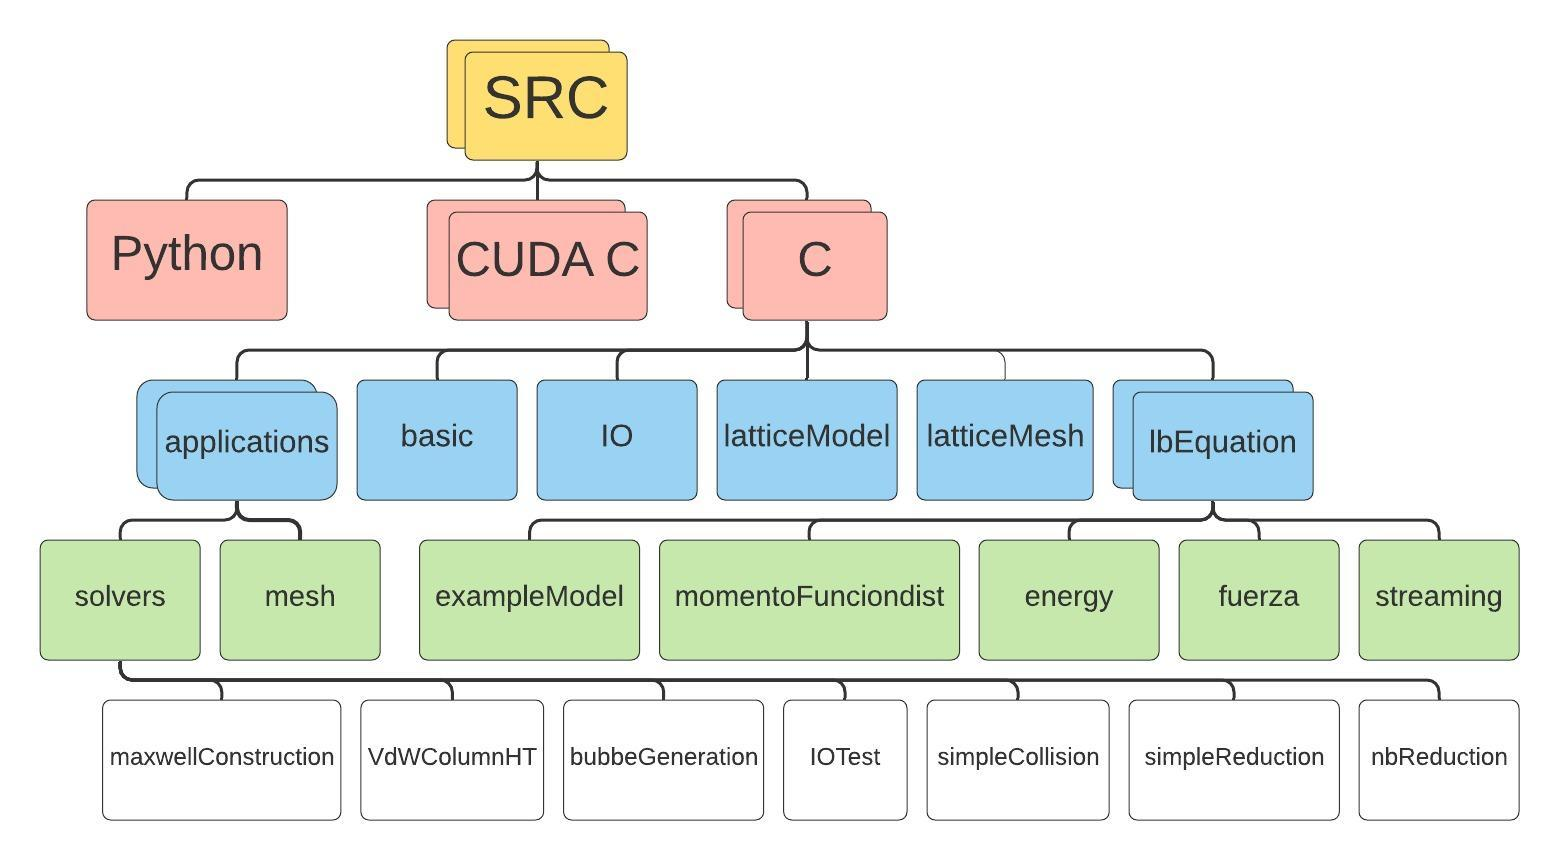
\includegraphics[width=\textwidth]{figs/cap3/arquitectura_del_proyecto_LBCUDA_Test}
	\caption{Esquema de la arquitectura del proyecto a partir del directorio SRC, el cual posee todos los códigos fuente. La carpeta de CUDA C presenta la misma estructura mostrada que la de C.}
	\label{fig:arq_proyecto}	
\end{figure}

\newpage

Cada una de las carpetas finales que se encuentran detalladas poseen uno o varios archivos que son funciones/\textit{kernels} con sus respectivos \textit{headers} y cada uno de los \textit{headers} tiene un \textit{link} simbólico en el directorio \textit{include}.

Para agregar las funciones o \textit{kernels} a las bibliotecas que se configuraron en el CMakeLists.text principal, se debe indicar una instrucción \textbf{add\_library()}. Primero se ejemplifica en el código de \textsc{C} para la biblioteca \textit{lbequation.so} con algunas de las funciones que posee la misma. En el directorio de lbEquation, además de contar con sus subdirectorios, posee un CMakeLists.txt el cual contiene la forma del siguiente archivo de configuración de \textsc{CMake} :

{\footnotesize
	\begin{frame}{}
		\lstset{language=c,
			framesep=2mm,
			%		baselinestretch=1.2,
			basicstyle=\ttfamily,
			keywordstyle=\color{blue}\ttfamily,
			stringstyle=\color{red}\ttfamily,
			commentstyle=\color{green}\ttfamily,
			morecomment=[l][\color{magenta}]{\#}
		}
		\begin{lstlisting}[frame=single]
#------------------ Generacion de bibliotecas ------------------#
		
		# Esquemas LB
		add_library(lbequation SHARED 
		exampleModel/exampleDensity.c
		...
		
		momentoFunciondist/momentoDensity.c
		
		fuerza/fuerzaPresionEOS.c
		...
		
		streaming/lbstreaming.c
		...
		
		energy/energyTemp.c
		...
		
		)
		\end{lstlisting}
		
	\end{frame}
}

En el caso del código de \textsc{Cuda C}, además de lo realizado, se debe agregar la instrucción de compilación en el formato \textsc{ptx} de cada uno de los \textit{kernels} desarrollados. El archivo de configuración de \textsc{CMake} de la siguiente página ejemplifica la forma de obtener lo requerido.

El directorio \textit{applications} posee archivos que contienen la definición de \textit{main} y son los ejecutables. Es necesario remarcar dos aspectos. Por un lado la estructuración de la memoria para resolver los problemas mediante el método descripto en la Sec. ( \ref{sec:LBM_2_ec_MRT}). Por otro lado la instrucción que debe dársele al compilador para que efectivamente el archivo sea compilado como un ejecutable.

\newpage
{\footnotesize
	\begin{frame}{}
		\lstset{language=c,
			framesep=2mm,
			%		baselinestretch=1.2,
			basicstyle=\ttfamily,
			keywordstyle=\color{blue}\ttfamily,
			stringstyle=\color{red}\ttfamily,
			commentstyle=\color{green}\ttfamily,
			morecomment=[l][\color{magenta}]{\#}
		}
		\begin{lstlisting}[frame=single]
# Biblioteca de pruebas para CUDA C/CXX
add_library(cudalbequation STATIC

cudaExampleModel/cudaExampleDensity.cu
...

cudaMomentoFunciondist/cudaMomentoDensity.cu
...

...

)

set_target_properties( cudalbequation 
		PROPERTIES CUDA_SEPARABLE_COMPILATION ON)

# Compilacion en PTX para uso de PyCUDA
add_library(cudalbequationPTX OBJECT

cudaExampleModel/cudaExampleDensity.cu
...

cudaMomentoFunciondist/cudaMomentoDensity.cu
...

...
)

set_property(TARGET cudalbequationPTX PROPERTY CUDA_PTX_COMPILATION ON)

install(TARGETS cudalbequationPTX
		OBJECTS DESTINATION ${CMAKE_SOURCE_DIR}/ptx )

		\end{lstlisting}
		
	\end{frame}
}

La estructura de la memoria utilizada, es reservada en matrices o vectores para todos los elementos de la malla con los parámetros que se detallan a continuación.

\begin{itemize}
	\item Función distribución de poblaciones \textit{f} y \textit{q}. (Tamaño N x q)
	\item un \textit{array} Swap para realizar el proceso de \textit{streaming}. (Tamaño N x q)
	\item información de elementos vecinos de un nodo de la malla (Tamaño N x q)
	\item Densidad $\rho$. (Tamaño N )
	\item Temperatura $T$. (Tamaño N )
	\item Velocidad $\mathbf{U}$. (Tamaño N x 3 )
	\item Fuerza de interacción entre elementos de malla $\mathbf{F_{int}}$. (Tamaño N x 3 )
	\item Fuerza de total actuante en los nodos $\mathbf{F_{tot}}$. (Tamaño N x 3 )
	
\end{itemize}

En éste caso \textit{N} es la cantidad de elementos de la malla y \textit{q} la dimensión de la velocidad de grilla del modelo.

Cabe destacar que la matriz que posee la información de los nodos vecinos, sigue una asignación utilizada según cómo está dispuesta la velocidad de grilla $\mathbf{e}$, como indica la Figura (\ref{fig:grilla_D2Q9}). En nuestro caso, la información se encuentra almacenada para el nodo \textit{i} de la siguiente forma:

\begin{align*}
	vecino_{\>i} =
	\begin{bmatrix}
	v_0 & v_1 & v_2 & v_3 & v_4 & v_6 & v_7 & v_8 \\
	\end{bmatrix}
\end{align*}

donde la nomeclatura de $v_\alpha$ indica que es el vecino que se encuentra en la dirección de $\alpha$. En el caso presentado $v_0 = i$. Ésta disposición marca la forma en que leerán los registros de memoria, pudiendo no estar optimizada totalmente.

Para finalizar se utiliza la instrucción \textbf{add\_exacutable()} y \textbf{target\_link\_libraries()} para realizar un archivo ejecutable mediante \textsc{CMake}. A modo de ejemplo, se muestra el archivo CMakeLists.txt del ejecutable maxwellConstruction que se encuentra en el directorio con su mismo nombre.

{\footnotesize
	\begin{frame}{}
		\lstset{language=c,
			framesep=2mm,
			%		baselinestretch=1.2,
			basicstyle=\ttfamily,
			keywordstyle=\color{blue}\ttfamily,
			stringstyle=\color{red}\ttfamily,
			commentstyle=\color{green}\ttfamily,
			morecomment=[l][\color{magenta}]{\#}
		}
		\begin{lstlisting}[frame=single]
#------------------ Construccion de Maxwell------------------#
# Construccion de Maxwell

add_executable(maxwellConstruction 
			"maxwellConstruction.c" "writeDebug.c")
target_link_libraries(maxwellConstruction 
			${PROJECT_LINK_LIBS} ${PROJECT_LINK_LIBS})

		
		\end{lstlisting}
		
	\end{frame}
}


Lo que se describió hasta la presente instancia es todo lo que se utilizó en cuanto a las instrucciones de compilación mediante la herramienta de software \textsc{CMake}. También se describió lo necesario para entender la estructuración del código y poder entender de forma clara, cómo es la aplicación de el método descripto en la Sec. (\ref{sec:LBM_2_ec_MRT}).

\newpage
\section{Control de versiones y desarrollo del código \\ numérico utilizando Git}
\label{sec:git}

Git es un software que sirve para controlar versiones de archivos que se encuentran en un repositorio. El mismo fue desarrollado por Linus Torvalds cuando él empezo a desarrollar el \textit{kernel} de \textit{Linux}. El proyecto de éste trabajo se desarrollo con el sistema operativo \textit{Debian 10} y se encuentra en el repositorio de la página web de \textsc{Git Hub}. El proyecto puede ser descargado mediante las siguientes líneas de comando en la terminal:

{\footnotesize
	\begin{frame}{}
		\lstset{language=bash,
			framesep=2mm,
			%		baselinestretch=1.2,
			basicstyle=\ttfamily,
			keywordstyle=\color{blue}\ttfamily,
			stringstyle=\color{red}\ttfamily,
			commentstyle=\color{green}\ttfamily,
			morecomment=[l][\color{magenta}]{\#}
		}
		\begin{lstlisting}
$ sudo apt-get install git #Para instalar Git

$ git clone https://github.com/efogliatto/LBCUDA_Test #Iniciar descarga 
		\end{lstlisting}
		
	\end{frame}
}

creándose un repositorio local del mismo.

\subsection{Conceptos básicos}

Para comprender el funcionamiento de \textit{git} se definen algunos conceptos básicos \cite{user:2020:git}. 

El estado de un repositorio indica los archivos añadidos al mismo, eliminados ó modificados. Añadir un archivo significa que \textit{git} realiza un seguimiento del mismo y su estado puede ser nuevo, modificado ó eliminado. Un \textit{commit} es indicarle a \textit{git} el estado actual que refleja el proyecto en todos sus archivos, por lo cual recibe una identificación, y al mismo se le asigna un comentario que debe reflejar las diferencias realizadas con respecto al estado anterior de los mismos. Una rama (\textit{branch}) es una línea de trabajo, donde se va realizando el proyecto añadiéndose \textit{commits}. Se pueden tener múltiples ramas para trabajar un proyecto y obtener un mejor desarrollo del mismo. Cuando es conveniente, una rama que terminó su desarrollo puede ser fusionada en otra, éste proceso se llama \textit{merge}.

\textit{Git} fue pensado para hacer desarrollo entre colaboradores. Lo más usual es contar con un repositorio remoto principal, en donde se encuentra el último estado del proyecto a trabajar. Cada uno de los colaboradores posee su propio repositorio, dependiendo de si es el propio o de otro colaborador recibe el nombre de local y remoto. Debido al trabajo contínuo de los colaboradores, el repositorio remoto puede ir variando. El proceso de colocar \textit{commits} que uno desarrolla en el repositorio remoto se llama \textit{push} y el de adquirir los \textit{commits} de otros colaboradores \textit{pull}.

\newpage
\subsection{Principales comandos}

En el transcurso del desarrollo del presente proyecto se utilizaron algunos de los comandos de \textit{git}. A continuación se detallan los más utilizados acompañados de una breve explicación. Para más información remitirse al manual de usuario que se encuentra en la siguiente página web \url{https://git-scm.com/docs/user-manual} o en su defecto directamente al libro \url{https://git-scm.com/book/en/v2}.

\begin{itemize}
	\item \textbf{git init}: inicializa un repositorio, también se puede hacer mediante la página \url{https://github.com} , entre varias plataformas existentes.
	\item \textbf{git add archivo}: se añade al repositorio el archivo de nombre \textit{archivo}
	\item \textbf{git status}: indica el estado actual del repositorio y la rama en la que se encuentra
	\item \textbf{git add *}: añade el estado actual de todos los archivos
	\item \textbf{git commit -a}: se realiza commit
	\item \textbf{git log}: se muestra los comentarios de todos los \textit{commits} realizados con su nombre indicatorio. Si se coloca \textbf{-n} como opción, se mostrarán los últimos n \textit{commits}.
	\item \textbf{git commit - -amend}: se utiliza cuando se realizo mal el comentario de un \textit{commit} o faltó agregar algún archivo.
	\item \textbf{git push}: se añade al repositorio remoto todos los \textit{commits} realizados.
	\item \textbf{git pull}: se bajan del repositorio remoto, los \textit{commits} que no se tienen en el local.
	\item \textbf{git checkout name}: el repositorio local vuelve al estado del nombre identifiatorio del \textit{commit}, sin perder lo trabajado.
	\item \textbf{git branch name\_branch}: si se desea modificar desde un cierto \textit{commit} se debe crear una nueva rama y a partir de ahí seguir el desarrollo, luego de ello se debe realizar \textbf{git checkout name\_branch}.
	\item \textbf{git diff}: posee varias opciones y nos muestra diferencias. Ellas pueden ser de un archivo de la rama actual, entre dos ramas, entre un archivo que se encuentra en dos ramas, entre otros.
	\item \textbf{git merge}: se utiliza para fusionar dos ramas. Si no hay conflictos entre las dos ramas que se fusionan se realiza un \textit{fast foward} y no se debe realizar nada. Si hay conflictos y no se realiza el \textit{merge} de forma automática, se debe resolver dicho conflicto. Remitirse al manual de usuario para mayor información.
\end{itemize}

\subsection{Buenas prácticas}

En el transcurso del proyecto se adquirieron buenas prácticas de desarrollo de código mediante \textit{git}, dónde algunas de ellas son las que se desarrollan a continuación.

\textbf{Commits}: al momento de realizar un commit, es recomendable no hacerlo sobre muchos archivos juntos, sino sobre algunos que reflejen un cambio en la misma línea de trabajo. El comentario que lleva el \textit{commit} debe ser corto y enfocado a un desarrollo o cambio puntual. Antes de hacer \textbf{push} al repositorio remoto verificar que todos los archivos que uno desea esten añadidos, caso contrario se los agrega y para no generar otro \textit{commit} es que se utiliza \textbf{git commit - -amend}.

\textbf{branchs}: para desarrollar mejor el proyecto y tener diferenciado como es su avance, es que se estila trabajar con diferentes niveles de ramas. Los niveles recomendados son tres (3), el primero es de la rama \textit{master} que posee la última versión estable, la segunda es la rama \textit{develop} donde se harán los desarrollos
 siendo de buena práctica tener una rama \textit{master} donde está la verción estable del proyecto, una rama \textit{develop} para desarrollar las modificaciones y una o varias ramas tipo \textit{feature} que se enfoca en desarrollar algo específico. La idea es que cuando se tengan terminadas las versiones del \textit{feature}, se realice en \textit{merge} a la rama \textit{develop} y una vez que ésta posea todos los \textit{feature} hacer un \textsc{merge} a la rama \textit{master}. Lo que se explico queda ilustrado mediante la Figura (\ref{fig:ramas}).
 
 \begin{figure}[htbp]
 	\centering
 	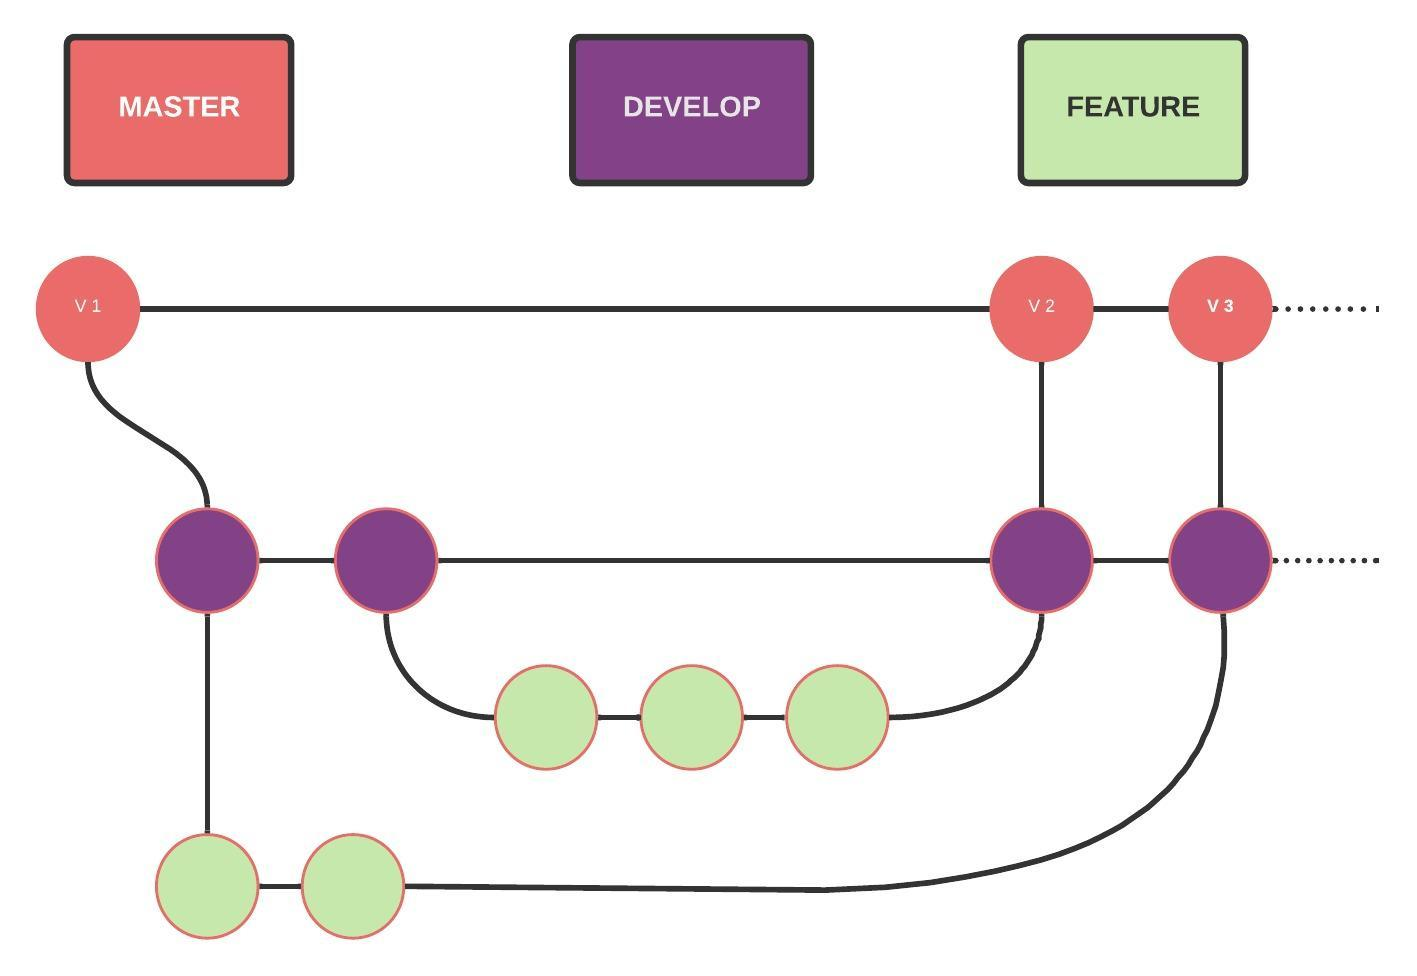
\includegraphics[width=0.85\textwidth]{figs/cap3/ejemplo_ramas}
 	\caption{Ejemplo de una buena práctica de la diagramación del proyecto mediante el uso de ramas.}
 	\label{fig:ramas}	
 \end{figure}
 
 


%Una vez creado un repositorio se debe indicar que se realice un seguimiento del mismo, para ello se utiliza el comando \textbf{git add (opciones)}, donde entre las opciones que se le puede indicar es el nombre del archivo a seguir.
%Si queremos er el estado de nuestro repositorio, se utiliza el comando \textbf{git status}, en dónde debe aparecer el archivo recientemente añadido a seguir. En el caso de que ése mismo archivo sea modificado ó eliminado, su estado será marcado al realizar \textbf{git status}. 

%Habiendose añadido todos los archivos que se deseean llevar al repositorio, es que se debe realizar un \textit{commit}, donde el mismo creará una imagen del estado actual del proyecto y a su vez se le debe iñadir un comentario haciendo alusión a lo que se realizó. Para ello es que se utiliza el comando \textbf{git commit -a} (pudiendo encontrarse otras opciones). Con el comando \textbf{git push} se añade a nuestro repositorio el \textit{commit} realizado.
%No es necesario que cada vez que se realice un \textit{commit} se suba al mismo al repositorio, es más, no es de buena práctica realizar ello, a menos que lo que se esté desarrollando lo amerite.



%Para saber el estado en que se encuentra el repositorio existe la función \textbf{git status}, que indicará si un archivo fue añadido, modificado ó eliminado. En el caso de que se desee hacer un seguimiento de todos los archivos listados mediante \textbf{git status}, se utiliza el comando \textbf{git add *}.


%%% Local Variables: 
%%% mode: latex
%%% TeX-master: "template"
%%% End: 

\chapter{Descripción de los problemas en fluidos con transferencia de calor }
\graphicspath{{figs/cap4/}}
\label{cap4}

En el presente capíulo se realiza la descripción de los problemas con transferencia de calor para fluidos multifásicos con cambio de fase llevados a cabo para validar los códigos numéricos desarrollados, siendo éstos la \textit{Construcción de Maxwell} y la \textit{Estratificación de un fluido Van Der Waals}

\section{Construcción de Maxwell}

Como se desarrollo en el Cap. \ref{cap2} la Ec. (\ref{eq:VdW_P}) es una EOS que modela el comportamiento de un gas real.

\begin{align*}
	P = \frac{R T}{V_m - b} - a {(\frac{1}{V_m})}^2
\end{align*}

La ecuación \ref{eq:VdW_P} puede ser representada gráficamente en un diagrama $P - V_m$. La figura \ref{fig:P_V_CO2} muestra el diagrama mencionado para el dióxido de carbono ($CO_2$) a distintas temperaturas: 373 (K), 304 (K) y 270 (K). Para $T = 270 \> K$ se vislumbra que en $p = 44,08 atm$ la gráfica se intersecta en tres valores de $V_m$, siendo dos de ellos estables. Por lo que se observa que hay dos volúmenes molares de coexistencia, indicando las fases líquido y gaseosa.

La construcción de Maxwell, también llamada regla de igualdad de áreas, indicada en la ecuación \ref{eq:maxwell_Construction}, es un procedimiento analítico para encontrar las densidades de coexistencia del líquido y gas. Donde $P$ es la presión de la EOS y $p_0$ es una presión constante. Al realizar la integral propuesta surge que las áreas A y B de la figura \ref{fig:P_V_CO2} deben ser iguales.

\begin{equation}
\int_{V_{m,l}}^{V_{m,g}} P d V_m = p_0 (V_{m,l} -  V_{m,g})
\label{eq:maxwell_Construction}
\end{equation}

\begin{figure}[h!]
	\centering
	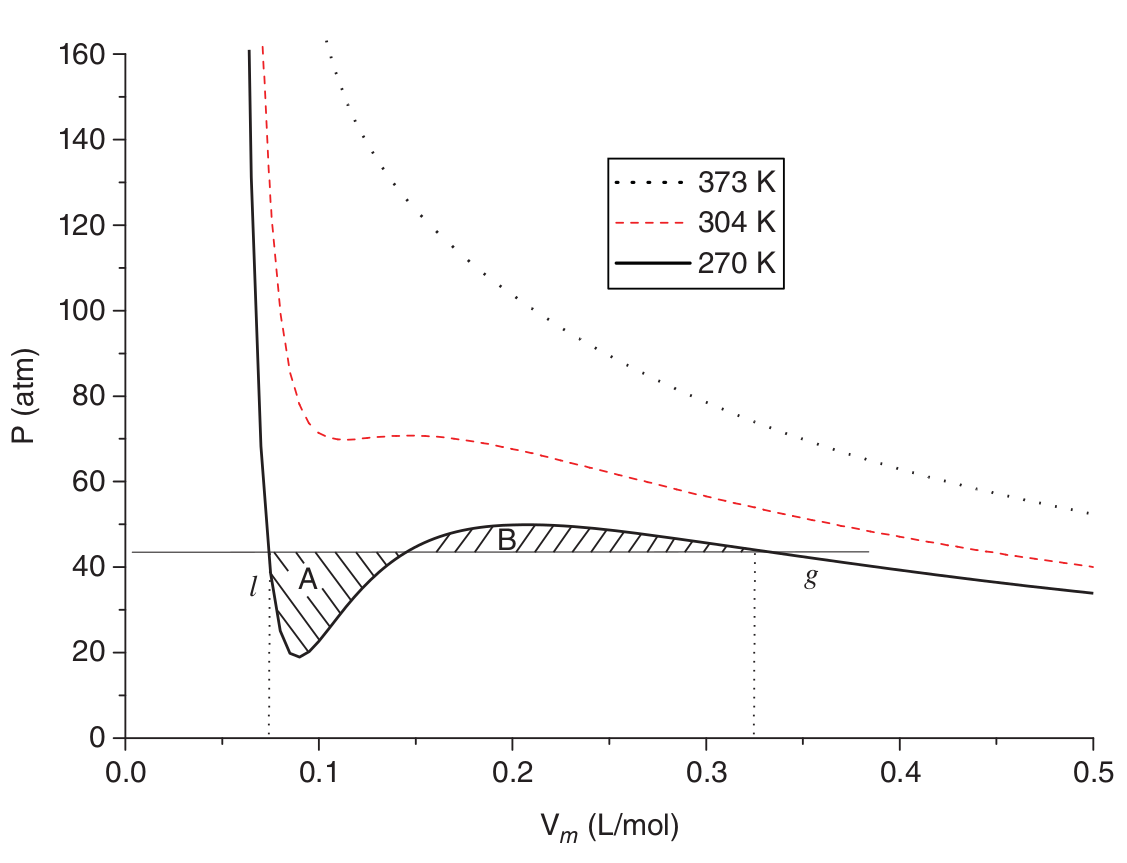
\includegraphics[width=.8\textwidth]{figs/cap2/Diagrama_P_V_del_CO2_Multiphase_LBM}
	\caption{Diagrama $P - V_m$ de la EOS de VdW del $CO_2$ con las constantes $a = 3,592$ y $b = 0,04267$, representando par a $T = 270 \> K$ los volúmenes molares del líquido y gas. \cite{huang2015multiphase}}
	\label{fig:P_V_CO2}	
\end{figure}


La EOS \ref{eq:VdW_P} se puede re-estructurar como \ref{eq:VdW_rho} puesto que $\rho = \frac{1}{v}$, siendo $v$ el volúmen másico y relacionando $V_m$ con $v$. Donde para un dado valor de temperatura tendremos la coexistencia de fases con su densidad $\rho_l$ para la fase líquida y $\rho_g$ para la gaseosa.

\begin{equation}
p = \frac{\rho R T}{1- \rho B} - A {\rho}^{2}
\label{eq:VdW_rho}
\end{equation}


\section{Estratificación de un fluido VdW con temperatura no uniforme}



\section{Generación de burbujas sobre una superficie horizontal calefaccionada}
%%% Local Variables: 
%%% mode: latex
%%% TeX-master: "template"
%%% End: 

\chapter{Conclusiones}
\graphicspath{{figs/cap4/}}
\label{cap5}

En el presente trabajo se realizaron dos códigos numéricos, desarrollados mediante los lenguajes de programación \textbf{C} y \textbf{CUDA C}, para resolver problemas de transferencia de calor en flujos multifásicos con cambio de fase.

El modelo utilizado es el de lattice Boltzmann de dos (2) ecuaciones pseudopotenciales con operador MRT, siédno el mismo del tipo D2Q9.

La validación del código se realizó en dos (2) GPU diferentes, siendo NVIDIA Geforce GTX 760 y  NVIDIA Geforce GTX 970; para simple precisión y doble precisión.

La validación se realizó por medio de tres (3) problemas físicos, siendo ellos:

\begin{itemize}
    
    \item la Construcción de Maxwell, el cuál obtiene las densidades de coexistencia de fases de un fluido 

    \item la estratificación de un fluido Van der Waals con temperatura no uniforme; siéndo el problema unidimensional con campo gravitatorio y temperaturas fijas en los extremos.

    \item la generación de burbujas en una placa horizontal calefaccionada.

\end{itemize}

\section{Construcción de Maxwell}

Para el problema de la Construcción de Maxwell, se reprodució el resultado que obtuvo Fogliatto en \cite{fogliatto2019simulation}, para el cuál el valor del parámetro $\sigma = 0,125$ del operador MRT es el que ajusta mejor la curva de coexistencia de fases para un fluido con la Ecuación de estado de VdW de parámetros $ a = 0,5 $ y $ b = 4,0 $. 

Para la GPU NVIDIA Geforce GTX 760 en simple precisión se obtuvo una ganancia del código realizado en \textbf{CUDA C} de 18.67 veces con respecto al código de \textbf{C} para un número de 64 \textit{thread block} y la cantidad de 4194304 ($2^{22}$) elementos de malla. Mientras que en la  GPU NVIDIA Geforce GTX 970 en las mismas condiciones se obtuvo una ganancia de 23.39 utilizando 32 \textit{thread block} .

En doble precisión, la ganancia de la GPU NVIDIA Geforce GTX 760 con 64 \textit{thread block} fue de 11.40 mientras que en GPU NVIDIA Geforce GTX 970 con 32 \textit{thread block} se obtuvo 10.96 .

Por el comportamiento que se observó en los resultados, la GPU NVIDIA Geforce GTX 760 llegó a una ganancia máxima, mientras que la GPU NVIDIA Geforce GTX 970 posee la tendencia de aumentar su ganancia a un número de elementos de malla mayor.

Se comparó los resultados obtenidos en simple precisión y doble precisión en la validación de las curvas de coexistencia. La comparación se hizo mediante la distancia de los vectores obtenidos de densidad con el vector de densidad analítico, calculándose la distancia como la norma euclídea. Se obtuvo que la diferencia entre la distancia en simple precisión es de 0,003 \% mayor que doble precisión.

Debido a que no existe un gran beneficio en la mejora que se obtiene utilizando doble precisión, y puesto que el tiempo que se demora en doble precesión con respecto a simple precisión es de 1.68 y 1.29 según se utilice GPU NVIDIA Geforce GTX 760/970 respectivamente. Se recomienda la utilización en simple precisión del código realizado.

\section{Estratificación de un fluido VdW}

Para el problema unidimensional de la estratificación de un fluido VdW, se pudo verificar los perfiles de densidad $\rho_r$ y de temperatura $T_r$ a lo largo de la cavidad. 

La mayor ganancia que se obtuvo para la GPU NVIDIA Geforce GTX 760 y GPU NVIDIA Geforce GTX 970 en simple precisión fue de 13.26 y 15.95; siendo para doble precisión en 7.88 y 13.29, tomando como comparación el código de \textsc{Cuda C} con el código de \textsc{C}. En todos los casos con 64 \textit{thread block}.

El código de \textsc{C} en simple precisión es 1.052 y 1.045 veces más rápida que en doble precisión; con las GPU NVIDIA Geforce GTX 760 GPU NVIDIA Geforce GTX 970 respectivamente. El código de \textsc{Cuda C} en simple precisión es 1.77 y 1.25 veces más rápida que en doble precisión; con las GPU NVIDIA Geforce GTX 760 y GPU NVIDIA Geforce GTX 970 respectivamente. En el caso del código en \textsc{C} es para 32 \textit{thread block}, siendo 64 \textit{thread block} en el código de \textsc{Cuda C}.

\newpage

\section{Generación de burbujas en una superficie horizontal calefaccionada}

A partir del problema de la estratificación de un fluido VdW con temperatura no uniforme, el cuál es unidimensional; se pudo realizar una pequeña modificación en el código, para agregar una condición de contorno de calefacción. En esencia el código es exactamente el mismo y puede reproducir el comportamiento de generación de una burbuja en el proceso de ebullición. 

Se demuestra de ésta manera que un fenómeno complejo puede ser resuelto mediante el LBM utilizado en el trabajo.

\section{Trabajo futuro}

Una de las líneas de desarrollo para éste trabajo es la mejora en los \textit{kernel} del código de \textsc{Cuda C} para que la ganancia en los tiempos de cálculo con respecto al del código de \textsc{C} aumente. Una de las formas de realizar ésto puede ser mediante la utilización de \textit{shared memory} ó \textit{local memory} de las \textit{thread block}. Por otro lado se puede trabajar en el desarrollo de una forma distinta de almacenar la información de los nodos vecinos; ya que cuando se realiza la lectura de los mismos no se utiliza toda la información y hay que ver la forma de que se almacenen de modo que cada vez que se lee el registro correspondiente de memoria se maximice la utilización de ésa lectura.

%Una de las cosas que queda por investigar , es el almacenamiento de los valores de la función de distribución de poblaciones, debido a que en nuestro problema se poseen 3 matrices con la información. una de ellas es la matriz de vecinosy la siguiente es las de poblaciones. Puesto a que depende de cómo es la etiqueta que se realizan a los vecinos, éstos irán a ser buscados en la memoria de la maquina. Dependiendo de cómo estén almacenados los lugares de la memoria de los nodos vecinos, éstos pueden tardart más o menios. de ahí surge la posibilidad/idea de que se distribuya de una manera distinta la forma de almacenar la informacion de lkis nodos vecinos y así realizzar un al profiling que haga que el código tenga una mayor ganancia.

Por cuestión de tiempo no se llegó a implementar un código en \textsc{Python} utilizando la biblioteca \textsc{PyCuda}. Se mostró la implementacion para uno de los \textit{kernel}, pudiendo continuar el proyecto a partir de ahí. 

También se puede realizar una interfaz gráfica mediante \textsc{Python} para que el usuario pueda operar el código sin necesidad de saber utilizar la terminal. La compilación del código puede realizarse de cierta forma, tal que se utilice en el sistema operativo Windows, ya que actualmente se utiliza en Linux. 

\appendix
%\chapter{Actividades relacionadas con la Práctica Profesional Supervisada y de Proyecto y Diseño}\label{ap1}
\graphicspath{{figs/}}

\section{Práctica profesional supervisada}

\section{Proyecto y diseño}

Las actividades de proyecto y diseño (PyD) realizadas para llevar a cabo el presente Proyecto Integrador de la carrera Ingeniería Nuclear fueron:
\begin{enumerate}
	\item Caracterización del diseño del SABR, desarrollada en el capítulo \ref{}.
	\item Validación del código OpenMC, detallada en el capítulo \ref{}.
	\item Cálculo del término fuente de neutrones debido a las reacciones de fusión, especificado en el capítulo \ref{}.
	\item Muestreo de la fuente externa de neutrones, indicado en el capítuo \ref{}.
	\item Cálculo neutrónico del reactor híbrido fusión-fisión, especificado en el capítulo \ref{}.
\end{enumerate}

%\chapter{}
\label{ap}

En el presente apéndice se muestra cuál es la matriz $\mathbf{M}$ en el modelo de LBM. También se encuentran diferenciados según el problema resuelto, los valores de $\mathbf{\Lambda}$ y $\mathbf{Q}$.

\begin{equation}
\mathbf{M} =
\begin{bmatrix}
	1 & 1 & 1 & 1 & 1 & 1 & 1 & 1 & 1 \\
   -4 &-1 &-1 &-1 &-1 & 2 & 2 & 2 & 2 \\
    4 &-2 &-2 &-2 &-2 & 1 & 1 & 1 & 1 \\
    0 & 1 & 0 &-1 & 0 & 1 &-1 &-1 & 1 \\
    0 &-2 & 0 & 2 & 0 & 1 &-1 &-1 & 1 \\
    0 & 0 & 1 & 0 &-1 & 1 & 1 &-1 &-1 \\
    0 & 0 &-2 & 0 & 2 & 1 & 1 &-1 &-1 \\
    0 & 1 &-1 & 1 &-1 & 0 & 0 & 0 & 0 \\    
    0 & 0 & 0 & 0 & 0 & 1 &-1 & 1 &-1 \\        
\end{bmatrix}
\end{equation}

\section{Construcción de Maxwell}
\label{parametros_MxC}

\begin{equation}
	diag(\mathbf{\Lambda}) = 
	\begin{bmatrix}
		1.0 & 0.8 & 1.1 & 1.0 & 1.1 & 1.0 & 1.1 & 0.8 & 0.8 \\
	\end{bmatrix}
\end{equation}

\begin{equation}
G = -1.0 \quad c = 1.0 \quad \sigma = 0.125 \quad a = 0.5 \quad b = 4.0 
\end{equation}

\begin{equation}
\mathbf{g} = (0.0 \quad 0.0 \quad 0.0 ) \qquad \rho_c = \frac{1}{12} \qquad T_c = 0.037037037
\end{equation}

\section{Estratificación de un fluido VdW}
\label{parametros_VdW}

\begin{equation}
	diag(\mathbf{\Lambda}) = 
	\begin{bmatrix}
		1.0 & 0.8 & 1.1 & 1.0 & 1.1 & 1.0 & 1.1 & 0.8 & 0.8 \\
	\end{bmatrix}
\end{equation}

\begin{equation}
diag(\mathbf{Q}) = 
	\begin{bmatrix}
		1.0 & 1.0 & 1.0 & 0.8 & 1.0 & 0.8 & 1.0 & 1.0 & 1.0 \\
	\end{bmatrix}
\end{equation}

\begin{equation}
	\alpha_{1} = 1.0 \qquad 	\alpha_{2} = 1.0 \qquad C_{v} = 1.0
\end{equation}

\begin{equation}
	G = -1.0 \quad c = 1.0 \quad \sigma = 0.125 \quad a = 0.5 \quad b = 4.0 
\end{equation}

\begin{equation}
\mathbf{g} = (0.0 \quad-1.234567e^{-7}\quad 0.0 ) \qquad \rho_c = \frac{1}{12} \qquad T_c = 0.037037037
\end{equation}

\section{Generación de burbujas}
\label{parametros_bub}

\begin{equation}
	diag(\mathbf{\Lambda}) = 
		\begin{bmatrix}
			1.0 & 1.25 & 1.0 & 1.0 & 1.1 & 1.0 & 1.1 & 1.3 & 1.3 \\
		\end{bmatrix}
\end{equation}

\begin{equation}
diag(\mathbf{Q}) = 
\begin{bmatrix}
1.0 & 1.0 & 1.0 & 1.55 & 1.0 & 1.55 & 1.0 & 1.0 & 1.0 \\
\end{bmatrix}
\end{equation}

\begin{equation}
\alpha_{1} = -2.0 \qquad 	\alpha_{2} = 2.0 \qquad C_{v} = 5.0
\end{equation}


\begin{equation}
G = -1.0 \quad c = 1.0 \quad \sigma = 0.125 \quad a = 1.0 \quad b = 4.0 
\end{equation}

\begin{equation}
\mathbf{g} = (0.0 \quad -8.0^{-6} \quad 0.0 ) \qquad \rho_c = \frac{1}{12} \qquad T_c = 0.074074074
\end{equation}
%\chapter{}
\label{ap1}

En el presente apéndice se encuentran las Tablas que contienen los valores de Speed Up entre el código realizado en C y CUDA C; para el problema de la Construcción de Maxwell.
Listándose para las dos placas gráficas utilizadas en el trabajo, diferenciándose en simple y doble precisión.
Además se encuentra la tabla que hace la comparación de Speed Up de simple y doble precisión según el código y la GPU utilizada.


\label{apend_MxC}

\title{\textbf{GPU NVIDIA GEFORCE GTX 760}}

\label{apend_MxC_760}

\begin{table}[h!]
\centering
    \begin{tabular}{|c|c|c|c|c|c|c|c|c|}
    \hline
                   & \multicolumn{8}{c|}{\textbf{NUMERO DE ELEMENTOS DE LA MALLA}} \\ \hline
    \textbf{BLOCK} & $2^{8}$ & $2^{10}$& $2^{12}$& $2^{14}$& $2^{16}$& $2^{18}$& $2^{20}$& $2^{22}$\\ \hline
    1              & 0.57  & 0.69  & 0.74  & 0.78  & 0.78  & 0.79  & 0.78  & 0.78  \\ \hline
    2              & 0.82  & 1.23  & 1.42  & 1.51  & 1.52  & 1.54  & 1.52  & 1.52  \\ \hline
    4              & 1.29  & 2.14  & 2.63  & 2.88  & 2.93  & 2.97  & 2.93  & 2.94  \\ \hline
    8              & 1.36  & 3     & 4.46  & 5.24  & 5.44  & 5.55  & 5.49  & 5.5   \\ \hline
    16             & 1.33  & 4.53  & 7.13  & 8.87  & 9.52  & 9.85  & 9.79  & 9.8   \\ \hline
    32             & 1.17  & 4.36  & 8.65  & 12.45 & 14.42 & 15.62 & 15.7  & 15.73 \\ \hline
    64             & 1.17  & 4.34  & 10.36 & 13.64 & 16.72 & 18.43 & 18.59 & 18.67 \\ \hline
    128            & 1.16  & 4.26  & 10.07 & 11.83 & 14.49 & 16.25 & 16.61 & 16.72 \\ \hline
    256            & 1.08  & 4.23  & 10.04 & 11.39 & 13.94 & 15.31 & 15.5  & 15.54 \\ \hline
    512            & 1.08  & 3.31  & 8.19  & 11.21 & 12.65 & 13.23 & 13.22 & 13.27 \\ \hline
    \end{tabular}
    \caption{Speed Up realizado para el problema de la Construcción de Maxwell con la GPU NVIDIA Geforce GTX 760 en simple precisión}
    \label{tab:s_760_MxC_simple_10}
    \end{table}

\begin{table}[h!]
\centering
    \begin{tabular}{|c|c|c|c|c|c|c|c|c|}
    \hline
                   & \multicolumn{8}{c|}{\textbf{NUMERO DE ELEMENTOS DE LA MALLA}} \\ \hline
    \textbf{BLOCK} & $2^{8}$ & $2^{10}$& $2^{12}$& $2^{14}$& $2^{16}$& $2^{18}$& $2^{20}$& $2^{22}$\\ \hline
    1              & 0.48  & 0.57  & 0.61  & 0.63  & 0.65  & 0.65  & 0.65  & 0.65  \\ \hline
    2              & 0.72  & 1.02  & 1.17  & 1.22  & 1.26  & 1.27  & 1.26  & 1.26  \\ \hline
    4              & 1.13  & 1.79  & 2.14  & 2.3   & 2.39  & 2.42  & 2.39  & 2.39  \\ \hline
    8              & 1.19  & 2.49  & 3.56  & 4.08  & 4.33  & 4.41  & 4.37  & 4.36  \\ \hline
    16             & 1.12  & 3.72  & 5.63  & 6.68  & 7.2   & 7.45  & 7.41  & 7.34  \\ \hline
    32             & 0.89  & 3.25  & 6.5   & 9     & 10.22 & 10.64 & 10.53 & 10.51 \\ \hline
    64             & 0.89  & 3.25  & 8.15  & 9.37  & 10.32 & 10.9  & 10.95 & 11.4  \\ \hline
    128            & 0.89  & 3.22  & 8.11  & 7.24  & 7.88  & 8.23  & 8.11  & 8.21  \\ \hline
    256            & 0.82  & 3.19  & 8.13  & 7.08  & 7.8   & 8.2   & 8.19  & 8.29  \\ \hline
    512            & 0.82  & 2.7   & 6.67  & 6.92  & 7.46  & 7.95  & 8.11  & 8.29  \\ \hline
    \end{tabular}
    \caption{Speed Up realizado para el problema de la Construcción de Maxwell con la GPU NVIDIA Geforce GTX 760 en doble precisión}
    \label{tab:s_760_MxC_double_10}
    \end{table}

% Please add the following required packages to your document preamble:
% \usepackage{multirow}
\begin{table}[]
    \begin{tabular}{|c|c|c|c|c|c|c|c|c|}
    \hline
    \multirow{2}{*}{} & \multicolumn{8}{c|}{\textbf{NUMERO DE ELEMENTOS DE LA MALLA}} \\ \cline{2-9} 
                      & $2^8$ & $2^10$& $2^12$& $2^14$& $2^16$& $2^18$& $2^20$& $2^22$\\ \hline
    \textbf{C}        &1.004  &1.003  &1.008  &1.000  &1.025  &1.023  &1.024  &1.026  \\ \hline
    \end{tabular}
    \caption{Speed Up realizado para el problema de la Construcción de Maxwell con la GPU NVIDIA Geforce GTX 760 en C comparando simple y doble precisión.}
    \label{tab:c_760_MxC_c_10}
    \end{table}

    


\begin{table}[h!]
    \begin{tabular}{|c|c|c|c|c|c|c|c|c|}
    \hline
                   & \multicolumn{8}{c|}{\textbf{NUMERO DE ELEMENTOS DE LA MALLA}} \\ \hline
    \textbf{BLOCK} & $2^8$ & $2^10$& $2^12$& $2^14$& $2^16$& $2^18$& $2^20$& $2^22$\\ \hline
    1              & 1.19  & 1.22  & 1.22  & 1.23  & 1.23  & 1.24  & 1.22  & 1.23  \\ \hline
    2              & 1.14  & 1.21  & 1.23  & 1.23  & 1.24  & 1.24  & 1.23  & 1.24  \\ \hline
    4              & 1.14  & 1.2   & 1.24  & 1.25  & 1.25  & 1.25  & 1.25  & 1.26  \\ \hline
    8              & 1.15  & 1.21  & 1.26  & 1.28  & 1.29  & 1.29  & 1.29  & 1.29  \\ \hline
    16             & 1.2   & 1.22  & 1.28  & 1.33  & 1.35  & 1.35  & 1.35  & 1.37  \\ \hline
    32             & 1.32  & 1.34  & 1.34  & 1.38  & 1.45  & 1.5   & 1.53  & 1.54  \\ \hline
    64             & 1.32  & 1.34  & 1.28  & 1.46  & 1.66  & 1.73  & 1.74  & 1.68  \\ \hline
    128            & 1.32  & 1.33  & 1.25  & 1.63  & 1.88  & 2.02  & 2.1   & 2.09  \\ \hline
    256            & 1.31  & 1.33  & 1.25  & 1.61  & 1.83  & 1.91  & 1.94  & 1.92  \\ \hline
    512            & 1.31  & 1.23  & 1.24  & 1.62  & 1.74  & 1.7   & 1.67  & 1.64  \\ \hline
    \end{tabular}
    \caption{Speed Up realizado para el problema de la Construcción de Maxwell con la GPU NVIDIA Geforce GTX 760 en CUDA comparando simple y doble precisión.}
    \label{tab:c_760_MxC_cuda_10}
    \end{table}


\newpage

\title{\textbf{GPU NVIDIA GEFORCE GTX 970}}

\label{apend_MxC_970}

\begin{table}[h!]
\begin{tabular}{|c|c|c|c|c|c|c|c|c|c|}
\hline
               & \multicolumn{9}{c|}{\textbf{NUMERO DE ELEMENTOS DE LA MALLA}}        \\ \hline
\textbf{BLOCK} & $2^8$& $2^10$& $2^12$& $2^14$& $2^16$& $2^18$& $2^20$& $2^22$& $2^24$\\ \hline
1              & 0.18 & 0.5   & 0.85  & 0.51  & 0.71  & 0.95  & 0.7   & 0.72  & 0.84  \\ \hline
2              & 0.24 & 0.71  & 1.43  & 0.81  & 1.3   & 1.96  & 1.74  & 1.47  & 1.28  \\ \hline
4              & 0.27 & 0.88  & 1.99  & 1.15  & 2.26  & 3.75  & 3.36  & 2.6   & 2.49  \\ \hline
8              & 0.27 & 0.7   & 0.7   & 1.44  & 3.97  & 6.8   & 6.39  & 5.13  & 5.32  \\ \hline
16             & 0.21 & 0.47  & 1.1   & 1.52  & 5.44  & 10.81 & 7.47  & 9.75  & 12.34 \\ \hline
32             & 0.22 & 0.78  & 2.02  & 1.54  & 7.1   & 14.5  & 9.96  & 13.68 & 23.39 \\ \hline
64             & 0.26 & 0.93  & 2.24  & 1.56  & 6.87  & 12.97 & 9.13  & 13.49 & 21.11 \\ \hline
128            & 0.27 & 0.93  & 2.16  & 1.79  & 6.84  & 8.32  & 9.07  & 11.81 & 17.23 \\ \hline
256            & 0.25 & 0.36  & 0.82  & 2.2   & 6.78  & 7.98  & 8.85  & 9.44  & 22.94 \\ \hline
512            & 0.15 & 0.37  & 0.95  & 1.74  & 6.2   & 7.67  & 8.74  & 9.21  & 21.68 \\ \hline
\end{tabular}
\caption{Speed Up realizado para el problema de la Construcción de Maxwell con la GPU NVIDIA Geforce GTX 970 en simple precisión}
\label{tab:s_970_MxC_simple_10}
\end{table}

\begin{table}[]
    \begin{tabular}{|c|c|c|c|c|c|c|c|c|}
    \hline
                   & \multicolumn{8}{c|}{\textbf{NUMERO DE ELEMENTOS DE LA MALLA}} \\ \hline
    \textbf{BLOCK} & $2^8$ & $2^10$& $2^12$& $2^14$& $2^16$& $2^18$& $2^20$& $2^22$\\ \hline
    1              & 0.16  & 0.41  & 0.67  & 0.7   & 0.49  & 0.57  & 0.54  & 0.53  \\ \hline
    2              & 0.23  & 0.61  & 1.21  & 1.26  & 0.91  & 1.38  & 1.03  & 1.09  \\ \hline
    4              & 0.25  & 0.86  & 1.64  & 2.16  & 1.67  & 2.84  & 2.24  & 2.01  \\ \hline
    8              & 0.25  & 0.66  & 0.68  & 3.15  & 2.65  & 4.95  & 4.84  & 3.95  \\ \hline
    16             & 0.19  & 0.39  & 0.84  & 2.34  & 3.66  & 8.14  & 8     & 7.15  \\ \hline
    32             & 0.2   & 0.7   & 1.54  & 1.48  & 4.29  & 10.06 & 9.38  & 10.96 \\ \hline
    64             & 0.25  & 0.89  & 1.98  & 1.48  & 3.93  & 8.02  & 7.44  & 8.29  \\ \hline
    128            & 0.25  & 0.89  & 1.92  & 1.48  & 3.92  & 7.98  & 7.41  & 8.39  \\ \hline
    256            & 0.24  & 0.34  & 0.83  & 1.48  & 3.91  & 7.93  & 7.38  & 6.34  \\ \hline
    512            & 0.13  & 0.3   & 1.15  & 1.47  & 4.54  & 7.98  & 6.16  & 6.33  \\ \hline
    \end{tabular}
    \caption{Speed Up realizado para el problema de la Construcción de Maxwell con la GPU NVIDIA Geforce GTX 970 en doble precisión}
    \label{tab:s_970_MxC_double_10}
    \end{table}

% Please add the following required packages to your document preamble:
% \usepackage{multirow}
\begin{table}[h!]
\centering
    \begin{tabular}{|c|c|c|c|c|c|c|c|c|}
    \hline
    \multirow{2}{*}{} & \multicolumn{8}{c|}{\textbf{NUMERO DE ELEMENTOS DE LA MALLA}} \\ \cline{2-9} 
                      & $2^{8}$ & $2^{10}$& $2^{12}$& $2^{14}$& $2^{16}$& $2^{18}$& $2^{20}$& $2^{22}$\\ \hline
    \textbf{C}        & 1.007 & 1.018 & 1.03  & 1.03  & 1.022 & 1.021 & 1.034 & 1.035 \\ \hline
    \end{tabular}
    \caption{Speed Up realizado para el problema de la Construcción de Maxwell con la GPU NVIDIA Geforce GTX 970 en C comparando simple y doble precisión.}
    \label{tab:c_970_MxC_c_10}
    \end{table}

\begin{table}[h!]
    \begin{tabular}{|c|c|c|c|c|c|c|c|c|}
    \hline
                   & \multicolumn{8}{c|}{\textbf{NUMERO DE ELEMENTOS DE LA MALLA}} \\ \hline
    \textbf{BLOCK} & $2^8$ & $2^10$& $2^12$& $2^14$& $2^16$& $2^18$& $2^20$& $2^22$\\ \hline
    1              & 1.13  & 1.22  & 1.3   & 0.76  & 1.48  & 1.7   & 1.36  & 1.42  \\ \hline
    2              & 1.06  & 1.19  & 1.21  & 0.67  & 1.46  & 1.45  & 1.75  & 1.41  \\ \hline
    4              & 1.07  & 1.04  & 1.25  & 0.55  & 1.38  & 1.35  & 1.55  & 1.34  \\ \hline
    8              & 1.06  & 1.07  & 1.07  & 0.47  & 1.53  & 1.4   & 1.37  & 1.34  \\ \hline
    16             & 1.1   & 1.21  & 1.34  & 0.67  & 1.52  & 1.36  & 0.96  & 1.41  \\ \hline
    32             & 1.1   & 1.13  & 1.35  & 1.08  & 1.69  & 1.47  & 1.1   & 1.29  \\ \hline
    64             & 1.07  & 1.07  & 1.16  & 1.08  & 1.79  & 1.65  & 1.27  & 1.68  \\ \hline
    128            & 1.05  & 1.06  & 1.16  & 1.24  & 1.79  & 1.07  & 1.26  & 1.46  \\ \hline
    256            & 1.06  & 1.07  & 1.02  & 1.53  & 1.77  & 1.03  & 1.24  & 1.54  \\ \hline
    512            & 1.16  & 1.23  & 0.85  & 1.21  & 1.39  & 0.98  & 1.47  & 1.51  \\ \hline
    \end{tabular}
    \caption{Speed Up realizado para el problema de la Construcción de Maxwell con la GPU NVIDIA Geforce GTX 970 en CUDA comparando simple y doble precisión.}
    \label{tab:c_970_MxC_cuda_10}
    \end{table}



%\chapter{}
\label{ap_VdW}

En el presente apéndice se encuentran las Tablas que contienen los valores de Speed Up entre el código realizado en C y CUDA C; para el problemas de la Estratificación de un fluido Van der Waals con temperatura no uniforme.
Listándose para las dos placas gráficas utilizadas en el trabajo, diferenciándose en simple y doble precisión.
Además se encuentra la tabla que hace la comparación de Speed Up de simple y doble precisión según el código y la GPU utilizada.\\
\\
\title{\textbf{GPU NVIDIA GEFORCE GTX 760}}
\label{apend_VdW_760}

\begin{table}[h!]
    \begin{tabular}{|c|c|c|c|c|c|c|c|c|c|c|c|c|c|c|}
    \hline
                   & \multicolumn{14}{c|}{\textbf{NUMERO DE ELEMENTOS DE LA MALLA}}                                                    \\ \hline
    \textbf{BLOCK} & 900  & 1200 & 2400 & 4800 & 9600 & 19200 & 38400 & 76800 & 153600 & 307200 & 614400 & 1228800 & 2457600 & 4915200 \\ \hline
    1              & 0.52 & 0.55 & 0.58 & 0.6  & 0.61 & 0.62  & 0.62  & 0.63  & 0.63   & 0.63   & 0.63   & 0.63    & 0.64    & 0.63    \\ \hline
    2              & 0.89 & 0.94 & 1.06 & 1.13 & 1.17 & 1.2   & 1.2   & 1.22  & 1.23   & 1.23   & 1.23   & 1.23    & 1.22    & 1.23    \\ \hline
    4              & 1.33 & 1.45 & 1.8  & 2.03 & 2.15 & 2.24  & 2.29  & 2.32  & 2.33   & 2.34   & 2.36   & 2.34    & 2.33    & 2.34    \\ \hline
    8              & 1.71 & 2.15 & 2.69 & 3.3  & 3.75 & 4.02  & 4.14  & 4.26  & 4.29   & 4.3    & 4.33   & 4.27    & 4.28    & 4.3     \\ \hline
    16             & 2.29 & 2.89 & 3.8  & 4.61 & 5.66 & 6.45  & 6.86  & 7.2   & 7.33   & 7.41   & 7.45   & 7.38    & 7.38    & 7.39    \\ \hline
    32             & 2.17 & 2.85 & 4.81 & 6.03 & 7.09 & 8.52  & 9.52  & 10.26 & 10.8   & 11.09  & 11.04  & 11.18   & 11.21   & 11.2    \\ \hline
    64             & 2.17 & 2.86 & 4.77 & 6.79 & 7.58 & 8.92  & 10.48 & 11.73 & 12.61  & 13.13  & 13.31  & 13.31   & 13.18   & 13.26   \\ \hline
    128            & 2.14 & 2.83 & 4.71 & 6.6  & 6.88 & 7.81  & 8.96  & 9.98  & 10.91  & 11.49  & 11.73  & 11.94   & 11.89   & 11.87   \\ \hline
    256            & 2.12 & 2.82 & 4.61 & 6.27 & 6.65 & 7.63  & 8.74  & 9.53  & 10.24  & 10.77  & 11.08  & 11.18   & 11.21   & 11.19   \\ \hline
    512            & 1.77 & 2.35 & 4.59 & 6.03 & 6.55 & 7.31  & 8.09  & 8.76  & 9.02   & 9.21   & 9.44   & 9.62    & 9.71    & 9.78    \\ \hline
    \end{tabular}
    \caption{Speed Up realizado para el problema de la Estratificación de Van der Waals con la GPU NVIDIA Geforce GTX 760 en simple precisión.}
    \label{tab:s_760_VdW_simple_10}
    \end{table}

\begin{table}[]
    \begin{tabular}{|c|c|c|c|c|c|c|c|c|c|c|c|c|c|c|}
    \hline
                                    & \multicolumn{14}{c|}{NUMERO DE ELEMENTOS DE LA MALLA}                                                             \\ \hline
    \textbackslash{}textbf\{BLOCK\} & 900  & 1200 & 2400 & 4800 & 9600 & 19200 & 38400 & 76800 & 153600 & 307200 & 614400 & 1228800 & 2457600 & 4915200 \\ \hline
    1                               & 0.42 & 0.44 & 0.46 & 0.48 & 0.49 & 0.49  & 0.5   & 0.52  & 0.51   & 0.52   & 0.52   & 0.51    & 0.52    & 0.53    \\ \hline
    2                               & 0.73 & 0.75 & 0.84 & 0.9  & 0.92 & 0.95  & 0.97  & 0.99  & 0.99   & 0.99   & 0.99   & 0.99    & 0.99    & 1.01    \\ \hline
    4                               & 1.08 & 1.16 & 1.41 & 1.58 & 1.67 & 1.74  & 1.8   & 1.84  & 1.85   & 1.86   & 1.85   & 1.84    & 1.85    & 1.88    \\ \hline
    8                               & 1.39 & 1.73 & 2.09 & 2.53 & 2.81 & 3.01  & 3.13  & 3.25  & 3.29   & 3.3    & 3.25   & 3.26    & 3.29    & 3.34    \\ \hline
    16                              & 1.86 & 2.33 & 2.98 & 3.5  & 4.17 & 4.7   & 5.01  & 5.23  & 5.31   & 5.4    & 5.37   & 5.32    & 5.33    & 5.43    \\ \hline
    32                              & 1.6  & 2.11 & 3.72 & 4.53 & 5.09 & 6.05  & 6.77  & 7.23  & 7.38   & 7.45   & 7.4    & 7.36    & 7.36    & 7.49    \\ \hline
    64                              & 1.6  & 2.12 & 3.72 & 5.05 & 5.39 & 6.16  & 6.77  & 7.21  & 7.51   & 7.79   & 7.91   & 7.95    & 7.96    & 7.88    \\ \hline
    128                             & 1.59 & 2.11 & 3.72 & 5    & 4.11 & 4.45  & 4.74  & 5.03  & 5.21   & 5.3    & 5.28   & 5.18    & 5.33    & 5.34    \\ \hline
    256                             & 1.59 & 2.1  & 3.71 & 4.75 & 4.02 & 4.5   & 4.7   & 4.98  & 5.19   & 5.28   & 5.28   & 5.23    & 5.32    & 5.3     \\ \hline
    512                             & 1.42 & 1.89 & 3.68 & 4.84 & 3.91 & 4.39  & 4.57  & 4.87  & 5.1    & 5.23   & 5.27   & 5.25    & 5.28    & 5.39    \\ \hline
    \end{tabular}
    \caption{Speed Up realizado para el problema de la Estratificación de Van der Waals con la GPU NVIDIA Geforce GTX 760 en doble precisión.}
    \label{tab:s_760_VdW_double_10}
    \end{table}

% Please add the following required packages to your document preamble:
% \usepackage{multirow}
\begin{table}[]
\begin{tabular}{|c|c|c|c|c|c|c|c|c|c|c|c|c|c|c|}
\hline
\multirow{2}{*}{} & \multicolumn{14}{c|}{\textbf{NUMERO DE ELEMENTOS DE LA MALLA}}                                                         \\ \cline{2-15} 
                  & 900   & 1200  & 2400  & 4800  & 9600  & 19200 & 38400 & 76800 & 153600 & 307200 & 614400 & 1228800 & 2457600 & 4915200 \\ \hline
\textbf{C}        & 1.001 & 0.999 & 1.002 & 1.006 & 1.003 & 1.007 & 1.023 & 1.033 & 1.031  & 1.031  & 1.032  & 1.031   & 1.033   & 1.052   \\ \hline
\end{tabular}
\caption{Speed Up realizado para el problema de la Estratificación de Van der Waals con la GPU NVIDIA Geforce GTX 970 en C comparando simple y doble precisión.}
\label{tab:c_760_VdW_c_10}
\end{table}

\begin{table}[h!]
\centering
\resizebox{17cm}{!}{
    \begin{tabular}{|c|c|c|c|c|c|c|c|c|c|c|c|c|c|c|}
    \hline
                   & \multicolumn{14}{c|}{\textbf{NUMERO DE ELEMENTOS DE LA MALLA}}                                                    \\ \hline
    \textbf{BLOCK} & 900  & 1200 & 2400 & 4800 & 9600 & 19200 & 38400 & 76800 & 153600 & 307200 & 614400 & 1228800 & 2457600 & 4915200 \\ \hline
    1              & 0.42 & 0.44 & 0.46 & 0.48 & 0.49 & 0.49  & 0.5   & 0.52  & 0.51   & 0.52   & 0.52   & 0.51    & 0.52    & 0.53    \\ \hline
    2              & 0.73 & 0.75 & 0.84 & 0.9  & 0.92 & 0.95  & 0.97  & 0.99  & 0.99   & 0.99   & 0.99   & 0.99    & 0.99    & 1.01    \\ \hline
    4              & 1.08 & 1.16 & 1.41 & 1.58 & 1.67 & 1.74  & 1.8   & 1.84  & 1.85   & 1.86   & 1.85   & 1.84    & 1.85    & 1.88    \\ \hline
    8              & 1.39 & 1.73 & 2.09 & 2.53 & 2.81 & 3.01  & 3.13  & 3.25  & 3.29   & 3.3    & 3.25   & 3.26    & 3.29    & 3.34    \\ \hline
    16             & 1.86 & 2.33 & 2.98 & 3.5  & 4.17 & 4.70  & 5.01  & 5.23  & 5.31   & 5.40   & 5.37   & 5.32    & 5.33    & 5.43    \\ \hline
    32             & 1.6  & 2.11 & 3.72 & 4.53 & 5.09 & 6.05  & 6.77  & 7.23  & 7.38   & 7.45   & 7.4    & 7.36    & 7.36    & 7.49    \\ \hline
    64             & 1.6  & 2.12 & 3.72 & 5.05 & 5.39 & 6.16  & 6.77  & 7.21  & 7.51   & 7.79   & 7.91   & 7.95    & 7.96    & 7.88    \\ \hline
    128            & 1.59 & 2.11 & 3.72 & 5    & 4.11 & 4.45  & 4.74  & 5.03  & 5.21   & 5.3    & 5.28   & 5.18    & 5.33    & 5.34    \\ \hline
    256            & 1.59 & 2.1  & 3.71 & 4.75 & 4.02 & 4.5   & 4.7   & 4.98  & 5.19   & 5.28   & 5.28   & 5.23    & 5.32    & 5.3     \\ \hline
    512            & 1.42 & 1.89 & 3.68 & 4.84 & 3.91 & 4.39  & 4.57  & 4.87  & 5.1    & 5.23   & 5.27   & 5.25    & 5.28    & 5.39    \\ \hline
    \end{tabular}}
    \caption{Speed Up realizado para el problema de la Estratificación de Van der Waals con la GPU NVIDIA Geforce GTX 760 en C comparando simple y doble precisión.}
    \label{tab:c_760_VdW_cuda_10}
    \end{table}

\newpage

\title{\textbf{GPU NVIDIA GEFORCE GTX 970}}
\label{apend_VdW_970}

\begin{table}[]
    \begin{tabular}{|c|c|c|c|c|c|c|c|c|c|c|c|c|c|c|}
    \hline
                   & \multicolumn{14}{c|}{\textbf{NUMERO DE ELEMENTOS DE LA MALLA}}                                                    \\ \hline
    \textbf{BLOCK} & 900  & 1200 & 2400 & 4800 & 9600 & 19200 & 38400 & 76800 & 153600 & 307200 & 614400 & 1228800 & 2457600 & 4915200 \\ \hline
    1              & 0.29 & 0.39 & 0.56 & 0.76 & 0.84 & 0.87  & 0.94  & 0.89  & 0.58   & 0.61   & 0.61   & 0.56    & 0.68    & 0.62    \\ \hline
    2              & 0.33 & 0.46 & 0.65 & 1.17 & 1.39 & 1.6   & 1.78  & 1.07  & 0.94   & 1      & 1.01   & 1.21    & 1.33    & 1.27    \\ \hline
    4              & 0.4  & 0.54 & 0.55 & 1.58 & 2.01 & 2.72  & 3.15  & 2.18  & 1.63   & 1.85   & 1.94   & 2.56    & 2.01    & 2.63    \\ \hline
    8              & 0.42 & 0.59 & 0.63 & 1.83 & 1.07 & 4.03  & 5.11  & 2.02  & 3.58   & 3.13   & 3.39   & 3.59    & 3.66    & 8.05    \\ \hline
    16             & 0.45 & 0.6  & 0.8  & 2.09 & 1.1  & 4.9   & 6.76  & 2.3   & 3.36   & 4.52   & 5.13   & 9.43    & 5.57    & 8.74    \\ \hline
    32             & 0.45 & 0.61 & 0.82 & 2.18 & 1.36 & 5.1   & 7.5   & 2.68  & 3.68   & 5.13   & 6.1    & 7.76    & 6.76    & 15.95   \\ \hline
    64             & 0.46 & 0.6  & 1    & 2.21 & 1.6  & 5.07  & 6.76  & 2.61  & 6.23   & 4.73   & 5.48   & 7.23    & 6.23    & 15.21   \\ \hline
    128            & 0.46 & 0.59 & 1    & 2.19 & 1.78 & 4.83  & 6.73  & 2.81  & 3.69   & 4.72   & 5.48   & 11.35   & 6.25    & 15.22   \\ \hline
    256            & 0.45 & 0.57 & 1.07 & 2.15 & 2.19 & 4.83  & 6.58  & 3.25  & 4.91   & 4.69   & 5.46   & 5.89    & 6.23    & 15.15   \\ \hline
    512            & 0.42 & 0.53 & 1.02 & 2.09 & 2.26 & 4.91  & 6.82  & 3.72  & 4.14   & 4.7    & 5.44   & 14.34   & 6.1     & 12.08   \\ \hline    \end{tabular}
    \caption{Speed Up realizado para el problema de la Estratificación de Van der Waals con la GPU NVIDIA Geforce GTX 970 en simple precisión.}
    \label{tab:s_970_VdW_simple_10}
    \end{table}

\begin{table}[]
    \begin{tabular}{|c|c|c|c|c|c|c|c|c|c|c|c|c|c|c|}
    \hline
                   & \multicolumn{14}{c|}{\textbf{NUMERO DE ELEMENTOS DE LA MALLA}}                                                    \\ \hline
    \textbf{BLOCK} & 900  & 1200 & 2400 & 4800 & 9600 & 19200 & 38400 & 76800 & 153600 & 307200 & 614400 & 1228800 & 2457600 & 4915200 \\ \hline
    \textbf{BLOCK} & 900  & 1200 & 2400 & 4800 & 9600 & 19200 & 38400 & 76800 & 153600 & 307200 & 614400 & 1228800 & 2457600 & 4915200 \\ \hline
    1              & 0.27 & 0.34 & 0.48 & 0.59 & 0.66 & 0.67  & 0.75  & 0.5   & 0.43   & 0.44   & 0.45   & 0.45    & 0.56    & 0.7     \\ \hline
    2              & 0.32 & 0.41 & 0.56 & 0.96 & 1.12 & 1.29  & 1.45  & 0.73  & 0.8    & 0.82   & 0.84   & 0.94    & 1.91    & 1.82    \\ \hline
    4              & 0.4  & 0.51 & 0.45 & 1.34 & 1.12 & 2.24  & 2.63  & 1.21  & 1.6    & 1.55   & 1.62   & 2.12    & 3.82    & 3.62    \\ \hline
    8              & 0.42 & 0.55 & 0.52 & 1.58 & 0.85 & 3.5   & 4.35  & 1.83  & 2.98   & 2.69   & 2.95   & 3.07    & 8.06    & 6.93    \\ \hline
    16             & 0.45 & 0.56 & 0.68 & 1.88 & 0.87 & 4.36  & 6.05  & 2.31  & 3.58   & 3.9    & 4.48   & 7.38    & 10.26   & 11.05   \\ \hline
    32             & 0.46 & 0.58 & 0.69 & 1.99 & 1.31 & 4.41  & 6.57  & 2.46  & 4.62   & 4.43   & 5.01   & 5.16    & 10.6    & 13.29   \\ \hline
    64             & 0.47 & 0.57 & 0.93 & 2.01 & 1.33 & 4.21  & 5.72  & 2.64  & 4.66   & 3.61   & 3.96   & 10.98   & 12.09   & 11.72   \\ \hline
    128            & 0.47 & 0.56 & 0.94 & 2    & 1.67 & 4.19  & 5.71  & 2.78  & 4.08   & 3.61   & 3.95   & 4.06    & 12.05   & 11.67   \\ \hline
    256            & 0.46 & 0.54 & 1.01 & 1.95 & 1.8  & 4.22  & 4.45  & 2.73  & 4.06   & 3.6    & 3.95   & 5.51    & 11.45   & 11.09   \\ \hline
    512            & 0.42 & 0.5  & 0.96 & 1.89 & 1.99 & 4.16  & 2.45  & 2.61  & 4.04   & 4.61   & 3.94   & 5.01    & 11.22   & 10.78   \\ \hline    \caption{Speed Up realizado para el problema de la Estratificación de Van der Waals con la GPU NVIDIA Geforce GTX 970 en doble precisión.}
    \label{tab:s_970_VdW_double_10}
    \end{table}

% Please add the following required packages to your document preamble:
% \usepackage{multirow}
\begin{table}[h!]
\centering
\resizebox{17cm}{!}{
\begin{tabular}{|c|c|c|c|c|c|c|c|c|c|c|c|c|c|c|}
\hline
\multirow{2}{*}{} & \multicolumn{14}{c|}{\textbf{NUMERO DE ELEMENTOS DE LA MALLA}}                                                         \\ \cline{2-15} 
                  & 900   & 1200  & 2400  & 4800  & 9600  & 19200 & 38400 & 76800 & 153600 & 307200 & 614400 & 1228800 & 2457600 & 4915200 \\ \hline
\textbf{C}        & 1.081 & 1.003 & 1.002 & 0.966 & 1.003 & 1.001 & 1.040 & 1.007 & 1.053  & 1.040  & 1.058  & 1.037   & 1.100   & 1.045   \\ \hline
\end{tabular}}
\caption{Speed Up realizado para el problema de la Estratificación de Van der Waals con la GPU NVIDIA Geforce GTX 970 en C comparando simple y doble precisión.}
\label{tab:c_970_VdW_c_10}
\end{table}

\begin{table}[]
    \begin{tabular}{|c|c|c|c|c|c|c|c|c|c|c|c|c|c|c|}
    \hline
                   & \multicolumn{14}{c|}{\textbf{NUMERO DE ELEMENTOS DE LA MALLA}}                                                    \\ \hline
    \textbf{BLOCK} & 900  & 1200 & 2400 & 4800 & 9600 & 19200 & 38400 & 76800 & 153600 & 307200 & 614400 & 1228800 & 2457600 & 4915200 \\ \hline
    1              & 1.15 & 1.14 & 1.18 & 1.24 & 1.27 & 1.3   & 1.29  & 1.79  & 1.44   & 1.45   & 1.45   & 1.31    & 1.32    & 0.92    \\ \hline
    2              & 1.11 & 1.12 & 1.16 & 1.18 & 1.24 & 1.24  & 1.28  & 1.47  & 1.24   & 1.27   & 1.27   & 1.33    & 0.76    & 0.73    \\ \hline
    4              & 1.07 & 1.07 & 1.23 & 1.14 & 1.81 & 1.21  & 1.24  & 1.81  & 1.07   & 1.24   & 1.26   & 1.25    & 0.58    & 0.76    \\ \hline
    8              & 1.06 & 1.07 & 1.21 & 1.12 & 1.26 & 1.15  & 1.22  & 1.11  & 1.26   & 1.21   & 1.22   & 1.21    & 0.5     & 1.21    \\ \hline
    16             & 1.07 & 1.07 & 1.18 & 1.07 & 1.27 & 1.12  & 1.16  & 1     & 0.99   & 1.2    & 1.21   & 1.33    & 0.6     & 0.83    \\ \hline
    32             & 1.07 & 1.06 & 1.19 & 1.06 & 1.04 & 1.16  & 1.19  & 1.1   & 0.84   & 1.2    & 1.29   & 1.56    & 0.7     & 1.25    \\ \hline
    64             & 1.07 & 1.05 & 1.08 & 1.06 & 1.21 & 1.21  & 1.23  & 1     & 1.41   & 1.36   & 1.47   & 0.68    & 0.57    & 1.36    \\ \hline
    128            & 1.06 & 1.05 & 1.06 & 1.06 & 1.07 & 1.16  & 1.23  & 1.02  & 0.95   & 1.36   & 1.47   & 2.9     & 0.57    & 1.36    \\ \hline
    256            & 1.06 & 1.05 & 1.05 & 1.06 & 1.22 & 1.15  & 1.54  & 1.2   & 1.27   & 1.35   & 1.46   & 1.11    & 0.6     & 1.43    \\ \hline
    512            & 1.06 & 1.06 & 1.06 & 1.06 & 1.14 & 1.18  & 2.9   & 1.44  & 1.08   & 1.06   & 1.46   & 2.97    & 0.6     & 1.17    \\ \hline    \end{tabular}
    \caption{Speed Up realizado para el problema de la Estratificación de Van der Waals con la GPU NVIDIA Geforce GTX 970 en CUDA comparando simple y doble precisión.}
    \label{tab:c_970_VdW_cuda_10}
    \end{table}



%\chapter{}
\label{ap_python}

En el presente apéndice se muestran los resultados obtenidos de un Speed Up al \textit{kernel} que calcula la densidad $\rho$ de la Ec.(\ref{eq:rho}) en la
GPU NVIDIA GEFORCE GTX 760 y GPU NVIDIA GEFORCE GTX 970, en los códigos de \textsc{C}, \textsc{Cuda C} y \textsc{Python}.

\begin{table}[h!]
\centering
    \begin{tabular}{|c|c|c|c|c|c|c|c|c|c|}
    \hline
                   & \multicolumn{9}{c|}{\textbf{NUMERO DE ELEMENTOS DE LA MALLA}} \\ \hline
    \textbf{BLOCK} & $2^{8}$ & $2^{10}$& $2^{12}$& $2^{14}$& $2^{16}$& $2^{18}$& $2^{20}$& $2^{22}$& $2^{24}$\\ \hline
		1                               & 0.193   & 0.389    & 0.365    & 0.302    & 0.325    & 0.348    & 0.345    & 0.347    & 0.347 \\ \hline
		2                               & 0.212   & 0.588    & 0.603    & 0.537    & 0.638    & 0.664    & 0.662    & 0.667    & 0.667 \\ \hline
		4                               & 0.158   & 0.549    & 0.836    & 1.009    & 1.068    & 1.243    & 1.236    & 1.243    & 1.242 \\ \hline
		8                               & 0.17    & 0.842    & 1.121    & 1.519    & 1.882    & 2.133    & 2.14     & 2.153    & 2.157 \\ \hline
		16                              & 0.197   & 0.775    & 1.303    & 1.953    & 2.653    & 3.054    & 3.101    & 3.132    & 3.135 \\ \hline
		32                              & 0.236   & 0.727    & 1.25     & 1.755    & 2.707    & 2.91     & 3.159    & 3.191    & 3.193 \\ \hline
		64                              & 0.244   & 0.591    & 1.262    & 1.833    & 2.425    & 3.124    & 3.164    & 3.195    & 3.198 \\ \hline
		128                             & 0.146   & 0.631    & 1.374    & 1.837    & 2.389    & 3.1      & 3.159    & 3.196    & 3.194 \\ \hline
		256                             & 0.165   & 0.751    & 1.187    & 1.701    & 2.373    & 3.107    & 3.157    & 3.181    & 3.194 \\ \hline
		512                             & 0.166   & 0.607    & 1.187    & 1.656    & 2.362    & 2.881    & 3.152    & 3.189    & 3.193 \\ \hline

    \end{tabular}
    \caption{Speed Up realizado entre CUDA y C para la función de colisión con la GPU NVIDIA Geforce GTX 760 en simple precisión}
    \label{tab:s_cuda_760_test_simple_10}
    \end{table}

\begin{table}[h!]
	\centering
	\begin{tabular}{|c|c|c|c|c|c|c|c|c|c|}
		\hline
		& \multicolumn{9}{c|}{\textbf{NUMERO DE ELEMENTOS DE LA MALLA}} \\ \hline
		\textbf{BLOCK} & $2^{8}$ & $2^{10}$& $2^{12}$& $2^{14}$& $2^{16}$& $2^{18}$& $2^{20}$& $2^{22}$& $2^{24}$\\ \hline
		1                               & 0.052   & 0.132    & 0.116    & 0.106    & 0.112    & 0.128    & 0.13     & 0.131    & 0.131 \\ \hline
		2                               & 0.055   & 0.167    & 0.183    & 0.196    & 0.239    & 0.26     & 0.254    & 0.257    & 0.258 \\ \hline
		4                               & 0.058   & 0.196    & 0.263    & 0.338    & 0.457    & 0.5      & 0.498    & 0.502    & 0.502 \\ \hline
		8                               & 0.06    & 0.234    & 0.358    & 0.523    & 0.808    & 0.925    & 0.937    & 0.945    & 0.946 \\ \hline
		16                              & 0.058   & 0.244    & 0.419    & 0.69     & 1.263    & 1.545    & 1.596    & 1.621    & 1.616 \\ \hline
		32                              & 0.055   & 0.241    & 0.46     & 0.802    & 1.586    & 2.026    & 2.118    & 2.162    & 2.168 \\ \hline
		64                              & 0.056   & 0.24     & 0.459    & 0.894    & 1.834    & 2.422    & 2.559    & 2.614    & 2.606 \\ \hline
		128                             & 0.058   & 0.239    & 0.477    & 0.889    & 1.988    & 2.628    & 2.608    & 2.8      & 2.867 \\ \hline
		256                             & 0.056   & 0.241    & 0.468    & 0.841    & 1.984    & 2.632    & 2.798    & 2.865    & 2.847 \\ \hline
		512                             & 0.059   & 0.225    & 0.448    & 0.848    & 2        & 2.619    & 2.786    & 2.856    & 2.866 \\ \hline
	\end{tabular}
	\caption{Speed Up realizado entre PyCUDA y C para la función de colisión con la GPU NVIDIA Geforce GTX 760 en simple precisión}
	\label{tab:s_py_c_760_test_simple_10}
\end{table}
\begin{table}[h!]
\centering
    \begin{tabular}{|c|c|c|c|c|c|c|c|c|c|}
    \hline
                   & \multicolumn{9}{c|}{\textbf{NUMERO DE ELEMENTOS DE LA MALLA}} \\ \hline
    \textbf{BLOCK} & $2^{8}$ & $2^{10}$& $2^{12}$& $2^{14}$& $2^{16}$& $2^{18}$& $2^{20}$& $2^{22}$& $2^{24}$\\ \hline
		1                               & 3.685   & 2.938    & 3.134    & 2.844    & 2.895    & 2.724    & 2.658    & 2.654    & 2.647 \\ \hline
		2                               & 3.853   & 3.525    & 3.299    & 2.74     & 2.668    & 2.558    & 2.603    & 2.596    & 2.584 \\ \hline
		4                               & 2.717   & 2.809    & 3.182    & 2.989    & 2.336    & 2.487    & 2.483    & 2.477    & 2.477 \\ \hline
		8                               & 2.842   & 3.601    & 3.131    & 2.904    & 2.329    & 2.306    & 2.285    & 2.277    & 2.28  \\ \hline
		16                              & 3.384   & 3.181    & 3.11     & 2.83     & 2.101    & 1.977    & 1.942    & 1.932    & 1.939 \\ \hline
		32                              & 4.297   & 3.014    & 2.717    & 2.189    & 1.707    & 1.436    & 1.492    & 1.476    & 1.473 \\ \hline
		64                              & 4.347   & 2.461    & 2.751    & 2.049    & 1.322    & 1.29     & 1.236    & 1.222    & 1.227 \\ \hline
		128                             & 2.525   & 2.646    & 2.881    & 2.066    & 1.202    & 1.18     & 1.211    & 1.141    & 1.114 \\ \hline
		256                             & 2.931   & 3.113    & 2.537    & 2.021    & 1.196    & 1.18     & 1.128    & 1.11     & 1.122 \\ \hline
		512                             & 2.792   & 2.696    & 2.652    & 1.953    & 1.181    & 1.1      & 1.132    & 1.117    & 1.114 \\ \hline
    \end{tabular}
    \caption{Speed Up realizado entre PyCUDA y CUDA para la función de colisión con la GPU NVIDIA Geforce GTX 760 en simple precisión}
    \label{tab:s_py_760_test_simple_10}
    \end{table}

\begin{table}[h!]
\centering
    \begin{tabular}{|c|c|c|c|c|c|c|c|c|c|}
    \hline
                   & \multicolumn{9}{c|}{\textbf{NUMERO DE ELEMENTOS DE LA MALLA}} \\ \hline
    \textbf{BLOCK} & $2^{8}$ & $2^{10}$& $2^{12}$& $2^{14}$& $2^{16}$& $2^{18}$& $2^{20}$& $2^{22}$& $2^{24}$\\ \hline
		1                               & 0.101   & 0.465    & 0.773    & 1.1      & 1.146    & 1.202    & 1.284    & 1.303    & 1.254 \\ \hline
		2                               & 0.106   & 0.52     & 1.047    & 1.837    & 2.115    & 2.605    & 2.885    & 2.569    & 2.474 \\ \hline
		4                               & 0.107   & 0.542    & 1.163    & 2.234    & 2.054    & 3.557    & 4.742    & 4.119    & 4.063 \\ \hline
		8                               & 0.107   & 0.547    & 1.269    & 2.39     & 3.529    & 4.331    & 4.679    & 4.616    & 4.307 \\ \hline
		16                              & 0.108   & 0.561    & 1.25     & 2.454    & 3.582    & 4.675    & 5.087    & 5.008    & 4.504 \\ \hline
		32                              & 0.105   & 0.553    & 1.245    & 2.468    & 3.645    & 4.716    & 4.944    & 4.658    & 4.67  \\ \hline
		64                              & 0.105   & 0.519    & 1.25     & 2.33     & 3.417    & 4.784    & 4.97     & 5.111    & 4.815 \\ \hline
		128                             & 0.102   & 0.56     & 1.249    & 2.578    & 3.395    & 4.77     & 5.37     & 4.753    & 4.578 \\ \hline
		256                             & 0.098   & 0.542    & 1.258    & 2.213    & 3.301    & 4.635    & 5.402    & 4.807    & 4.685 \\ \hline
		512                             & 0.099   & 0.496    & 1.287    & 2.479    & 3.46     & 4.74     & 5.397    & 5.052    & 4.592 \\ \hline
    \end{tabular}
    \caption{Speed Up realizado entre CUDA y C para la función de colisión con la GPU NVIDIA Geforce GTX 970 en simple precisión}
    \label{tab:s_cuda_970_test_simple_10}
    \end{table}

\begin{table}[h!]
	\centering
	\begin{tabular}{|c|c|c|c|c|c|c|c|c|c|}
		\hline
		& \multicolumn{9}{c|}{\textbf{NUMERO DE ELEMENTOS DE LA MALLA}} \\ \hline
		\textbf{BLOCK} & $2^{8}$ & $2^{10}$& $2^{12}$& $2^{14}$& $2^{16}$& $2^{18}$& $2^{20}$& $2^{22}$& $2^{24}$\\ \hline
		1                               & 0.025   & 0.093    & 0.131    & 0.162    & 0.181    & 0.187    & 0.217    & 0.213    & 0.200 \\ \hline
		2                               & 0.031   & 0.137    & 0.217    & 0.299    & 0.388    & 0.396    & 0.438    & 0.435    & 0.421 \\ \hline
		4                               & 0.033   & 0.162    & 0.31     & 0.496    & 0.722    & 0.719    & 0.847    & 0.849    & 0.771 \\ \hline
		8                               & 0.033   & 0.173    & 0.374    & 0.734    & 1.166    & 1.273    & 1.404    & 1.460    & 1.327 \\ \hline
		16                              & 0.033   & 0.188    & 0.451    & 0.995    & 1.723    & 1.929    & 2.188    & 2.277    & 2.064 \\ \hline
		32                              & 0.032   & 0.184    & 0.474    & 1.244    & 2.266    & 2.432    & 3.081    & 3.133    & 2.831 \\ \hline
		64                              & 0.033   & 0.178    & 0.453    & 1.386    & 2.74     & 3.013    & 3.972    & 3.532    & 3.507 \\ \hline
		128                             & 0.034   & 0.177    & 0.494    & 1.334    & 2.934    & 3.913    & 4.598    & 4.059    & 4.025 \\ \hline
		256                             & 0.03    & 0.171    & 0.489    & 1.335    & 2.966    & 3.307    & 4.701    & 4.683    & 4.242 \\ \hline
		512                             & 0.031   & 0.174    & 0.46     & 1.347    & 2.926    & 3.177    & 4.495    & 4.376    & 4.226 \\ \hline
	\end{tabular}
	\caption{Speed Up realizado entre PyCUDA y C para la función de colisión con la GPU NVIDIA Geforce GTX 970 en simple precisión}
	\label{tab:s_py_c_970_test_simple_10}
\end{table}

\begin{table}[t!]
\centering
    \begin{tabular}{|c|c|c|c|c|c|c|c|c|c|}
    \hline
                   & \multicolumn{9}{c|}{\textbf{NUMERO DE ELEMENTOS DE LA MALLA}} \\ \hline
    \textbf{BLOCK} & $2^{8}$ & $2^{10}$& $2^{12}$& $2^{14}$& $2^{16}$& $2^{18}$& $2^{20}$& $2^{22}$& $2^{24}$\\ \hline
		1                               & 4.016   & 5.016    & 5.886    & 6.799    & 6.342    & 6.412    & 5.912    & 6.12     & 6.266 \\ \hline
		2                               & 3.405   & 3.805    & 4.814    & 6.14     & 5.456    & 6.586    & 6.585    & 5.907    & 5.879 \\ \hline
		4                               & 3.265   & 3.353    & 3.752    & 4.503    & 2.846    & 4.948    & 5.597    & 4.85     & 5.271 \\ \hline
		8                               & 3.273   & 3.166    & 3.393    & 3.257    & 3.026    & 3.404    & 3.333    & 3.161    & 3.245 \\ \hline
		16                              & 3.253   & 2.983    & 2.77     & 2.467    & 2.079    & 2.423    & 2.325    & 2.2      & 2.182 \\ \hline
		32                              & 3.284   & 3.016    & 2.63     & 1.984    & 1.608    & 1.939    & 1.605    & 1.487    & 1.65  \\ \hline
		64                              & 3.199   & 2.911    & 2.756    & 1.68     & 1.247    & 1.588    & 1.251    & 1.447    & 1.373 \\ \hline
		128                             & 3.042   & 3.167    & 2.525    & 1.933    & 1.157    & 1.219    & 1.168    & 1.171    & 1.137 \\ \hline
		256                             & 3.237   & 3.165    & 2.574    & 1.658    & 1.113    & 1.402    & 1.149    & 1.026    & 1.104 \\ \hline
		512                             & 3.179   & 2.851    & 2.796    & 1.841    & 1.182    & 1.492    & 1.201    & 1.154    & 1.087 \\ \hline
    \end{tabular}
    \caption{Speed Up realizado entre PyCUDA y CUDA para la función de colisión con la GPU NVIDIA Geforce GTX 970 en simple precisión}
    \label{tab:s_py_970_test_simple_10}
    \end{table}


\begin{biblio}
\bibliography{biblio}
\end{biblio}


\begin{postliminary}

\listoffigures                  %Figuras

\listoftables                   %Tablas

\begin{seccion}{Agradecimientos}
\begin{small}	

Inserte aquí su agradecimiento.

\end{small}


\end{seccion}


\end{postliminary}



\end{document}
